\section{Preprocessing}
La base de dades de la que es va partir ja estava preprocessada degut al treball realitzat en anys anteriors. Per aquest motiu, per tal de poder comparar diferents mètodes d'imputació s'han hagut d'assignar valors mancants.

Per afegir valors mancants, s'ha determinat que, tenint en compte les característiques de la base de dades, les millors variables per contenir missings i poder imputar-los correctament són \textit{danceability}, \textit{speechiness} i \textit{duration}. Per tant, s'ha afegir aproximadament un 4\% de missing data en aquestes columnes. A més, com que en aquesta base de dades hi ha múltiples files que representen una mateixa cançó (cada una en una setmana diferent), s'ha assegurat que quan s'afegís un valor mancant en una instància d'una cançó, també s'afegís a la resta d'aparicions d'aquesta mateixa cançó, per tal de que els missings siguin coherents.

Finalment, per poder assegurar que els missings han estat afegits de manera aleatòria, s'ha realitzat el test de Little. En aquest test, la hipòtesis nul·la ($H_0$) és que les dades són MCAR (Missing Completely At Random), indicant que els valors mancants són totalment han estat afegits de forma totalment aleatòria. Els resultats d'aquest test han donat un $\textit{p-valor} > 0.05$, indicant que no hi ha suficient evidència estadística per poder descartar la hipòtesis nul·la, de manera que podem considerar que els valors mancants afegits són completament aleatoris (MCAR).

\subsection{Imputació de valors mancants}
Després de validar que, efectivament, el \textit{missing data} era aleatori, es va procedir amb la imputació mitjançant amb 3 mètodes diferents:

\subsubsection{MIMMI}

MIMMI és un mètode d'imputació descrit en \cite{gibert_2013_mixed}, on s'utilitza un clústering per imputar els valors mancants. Per aquest motiu, el mètode ens demana que escollim una k per triar quants clústers volem. El dendrograma del clústering, usant la mètrica de Gower i el mètode de Ward.D2 era el següent (\ref{fig:Preprocessing_mimmi_dend}):

\begin{figure}[H]
    \centering
    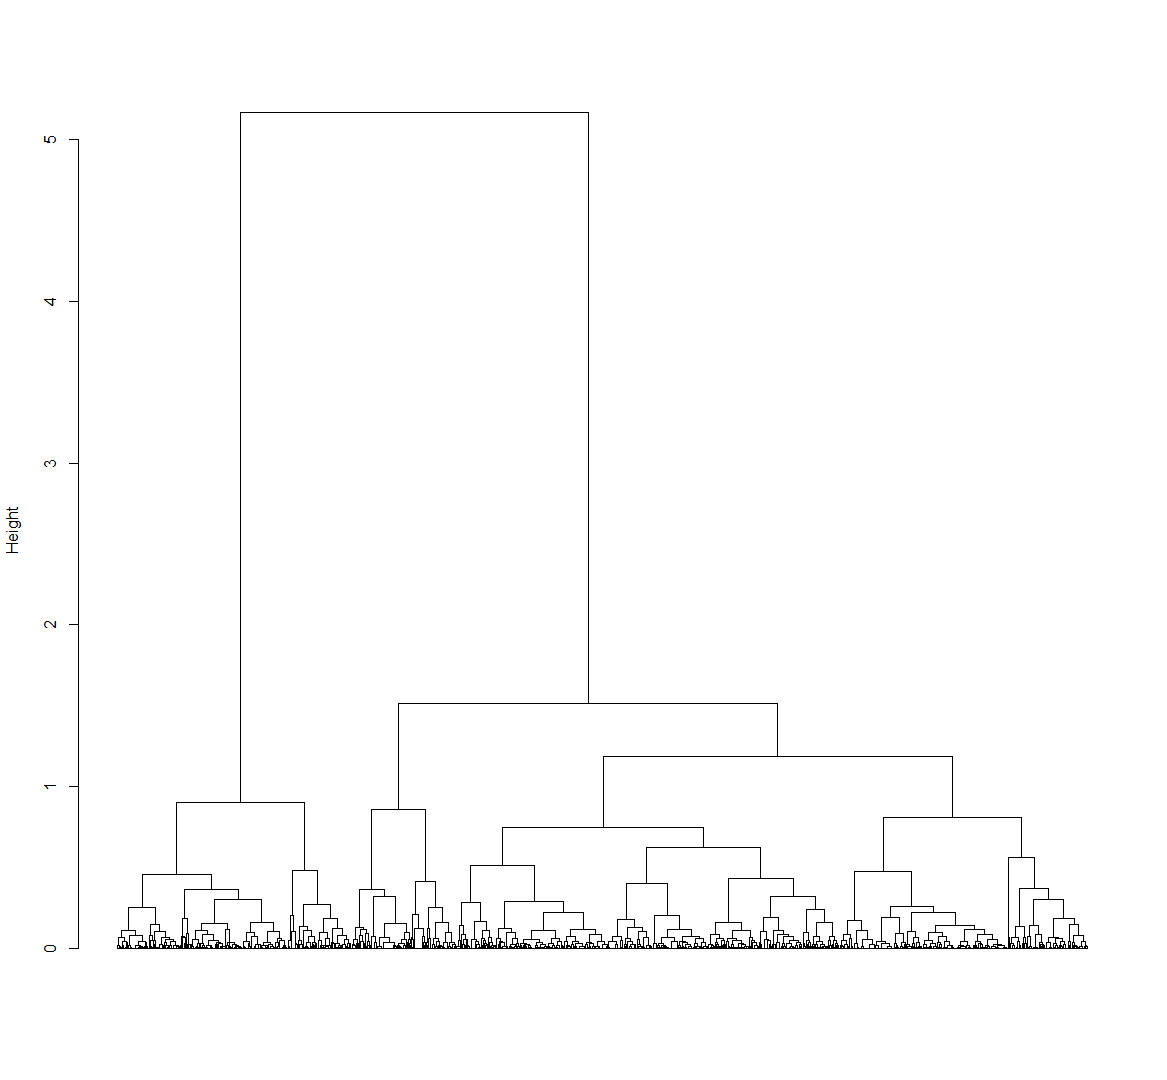
\includegraphics[width=0.8\textwidth]{Images/3_Preprocessing/mimmidend.png}
    \caption{Dendrograma usat pel MIMMI}
    \label{fig:Preprocessing_mimmi_dend}
\end{figure}

En aquest cas, vam escollir k = 4. Amb aquests clústers, realitzats amb les dades que no contenen missing data, es pot imputar la resta de instàncies simplement observant quin és el clúster que els hi pertoca i realitzant la mitja (o la moda, tot i que en aquest cas només s'han imputat variables numèriques).

\subsubsection{MICE} 
\textit{Multivariate Imputation by Chained Equations} (\cite{stefvanbuuren_2000_multivariate}), més conegut com MICE, és un altre mètode d'imputació. En aquest, es produeixen múltiples imputacions per variable que es combinen per obtenir el resultat final. Els paràmetres que es van usar per utilitzar-lo en la base de dades van ser: \textit{predictive mean matching} com a mètode (pmm), m (número de imputacions múltiples) 5 i màxim 5 iteracions.

R disposa d'un paquet amb aquest mètode, o sigui que la implementació ja estava feta.

\subsubsection{KNN}

Per imputar les dades usant KNN, s'han utilitzat tan sols les variables numèriques. S'han usat les variables completes (\textit{track\_popularity, album\_popularity, artist\_popularity, artist\_num, energy, loudness, acousticness, liveness, valence, tempo} i \textit{streams}) com a referència.

Per poder imputar, s'han usat com a train les instàncies del dataset amb aquestes variables on el dataset original no contenia missings a la variable a imputar. La "classificació" d'aquest train eren els valors de la variable a imputar (que no tenien missing). Llavors, com a test, s'usen la resta, que són els que contenen missing. D'aquesta manera es poden afegir aquests valors mancants usant el KNN. El valor de k usat ha estat el per defecte, 1, i la distància euclidiana (també el valor per defecte).

Després de les 3 imputacions, la suma total dels valors mancants del dataset era 420. Aquests, però, corresponen a valors mancants en les variables categòriques, especialment en aquelles provinents de APIs ja que va haver-hi alguns problemes. Més endavant s'explicarà com es van sol·lucionar aquests errors.


\subsection{Anàlisi descriptiva post processat}

Després del preprocessament, no quedaven categories incorrectes ni valors mancants. Degut a això, algunes distribucions canviaven. El primer que farem, però, per poder avaluar els diferents mètodes d'imputació, és comparar les distirbucions en les variables numèriques que han quedat. Per això, observem les diferències en les distribucions després d'imputar (figures \ref{fig:Preprocessing_distribdance}, \ref{fig:Preprocessing_distribduration} i \ref{fig:Preprocessing_distribspeech}).

\begin{figure}[H]
    \centering
    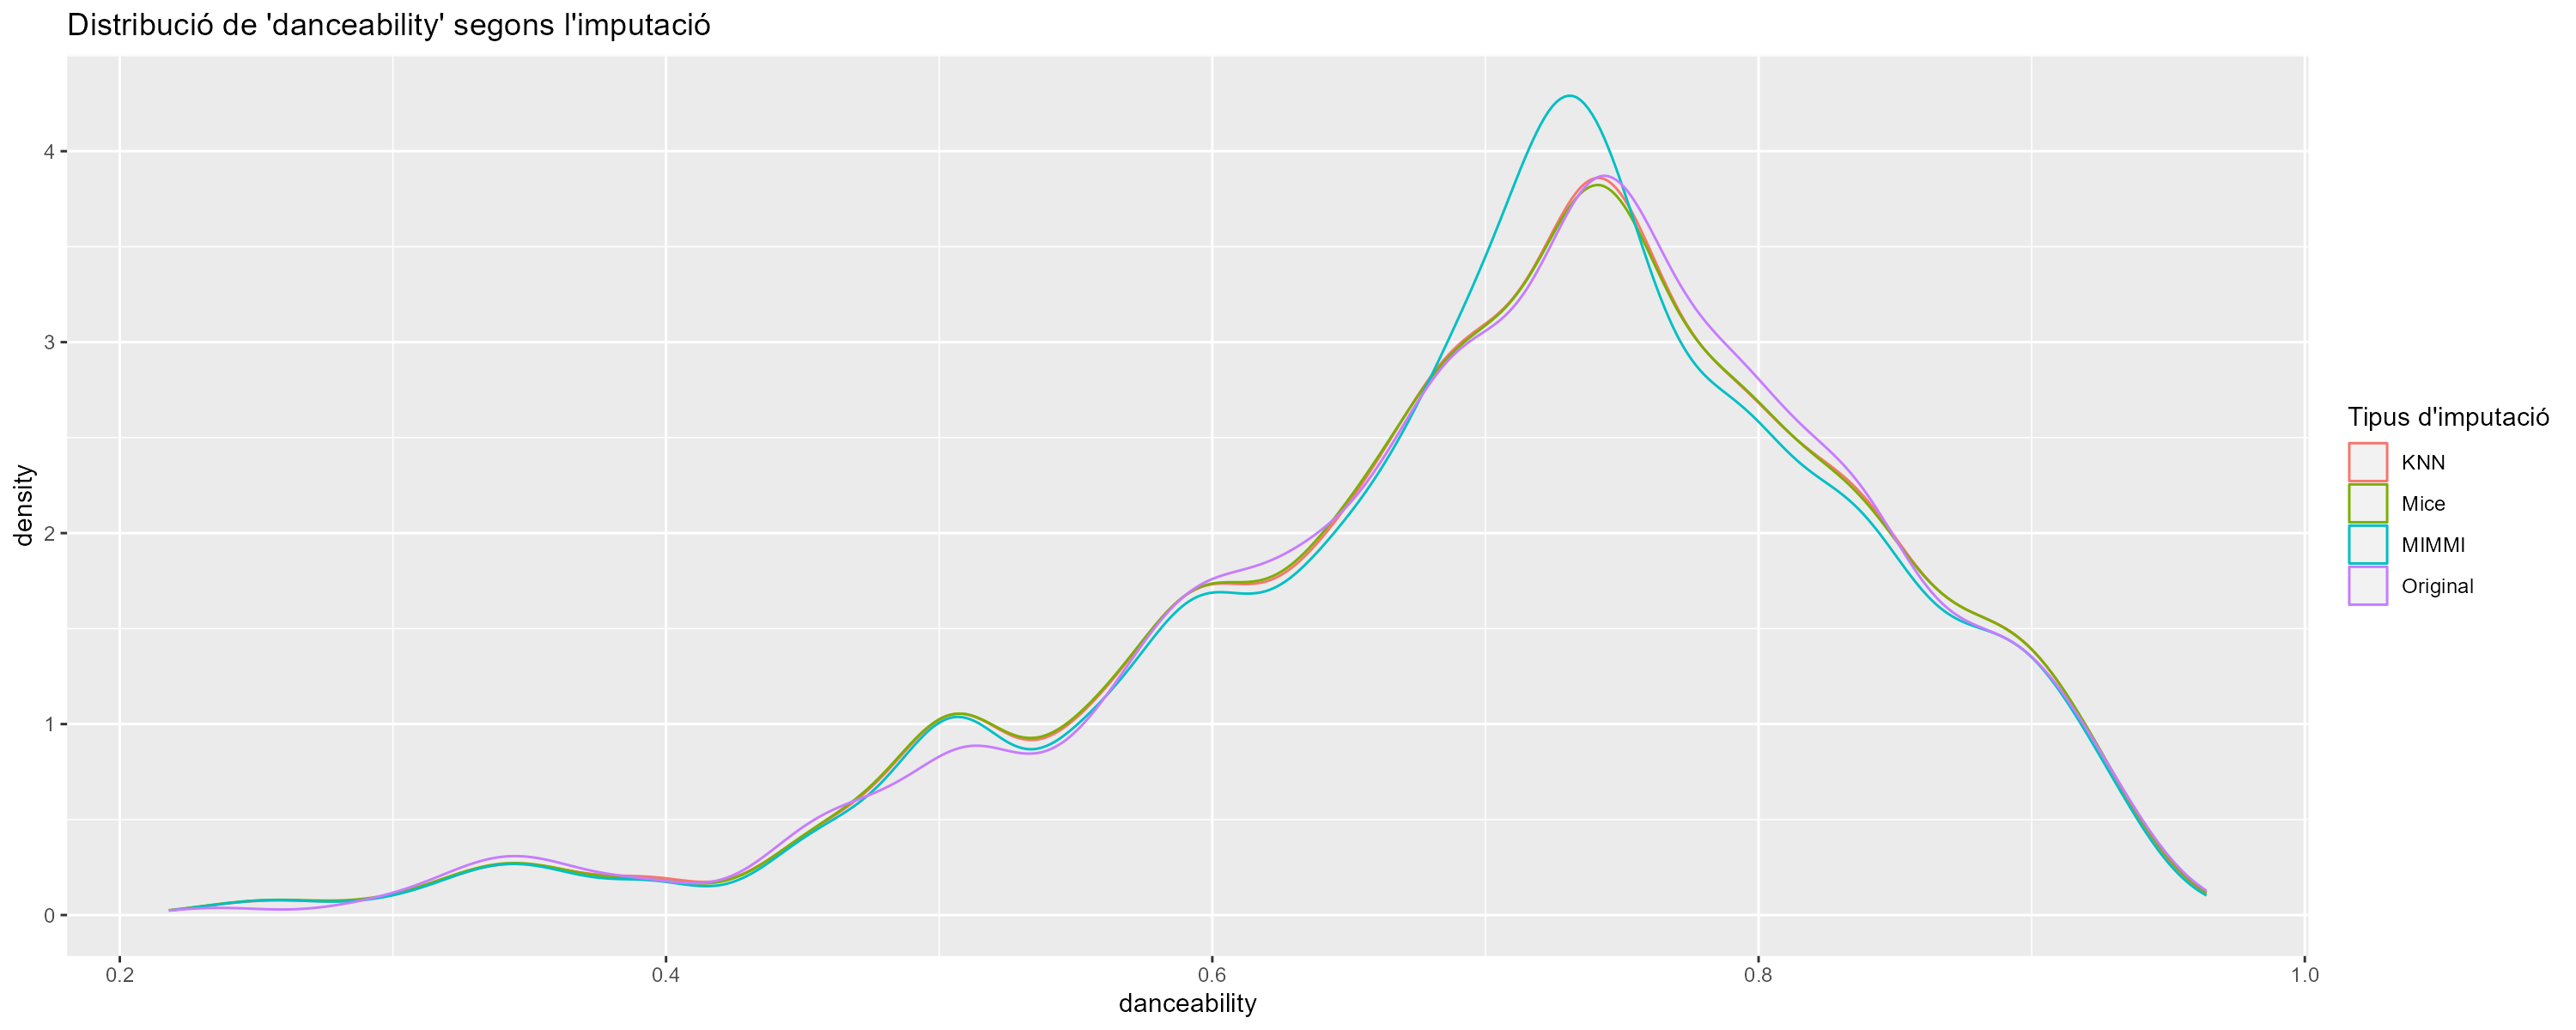
\includegraphics[width=0.8\textwidth]{Images/3_Preprocessing/distrib_imputation_danceability.png}
    \caption{Distribucions de danceability després de la imputació}
    \label{fig:Preprocessing_distribdance}
\end{figure}

\begin{figure}[H]
    \centering
    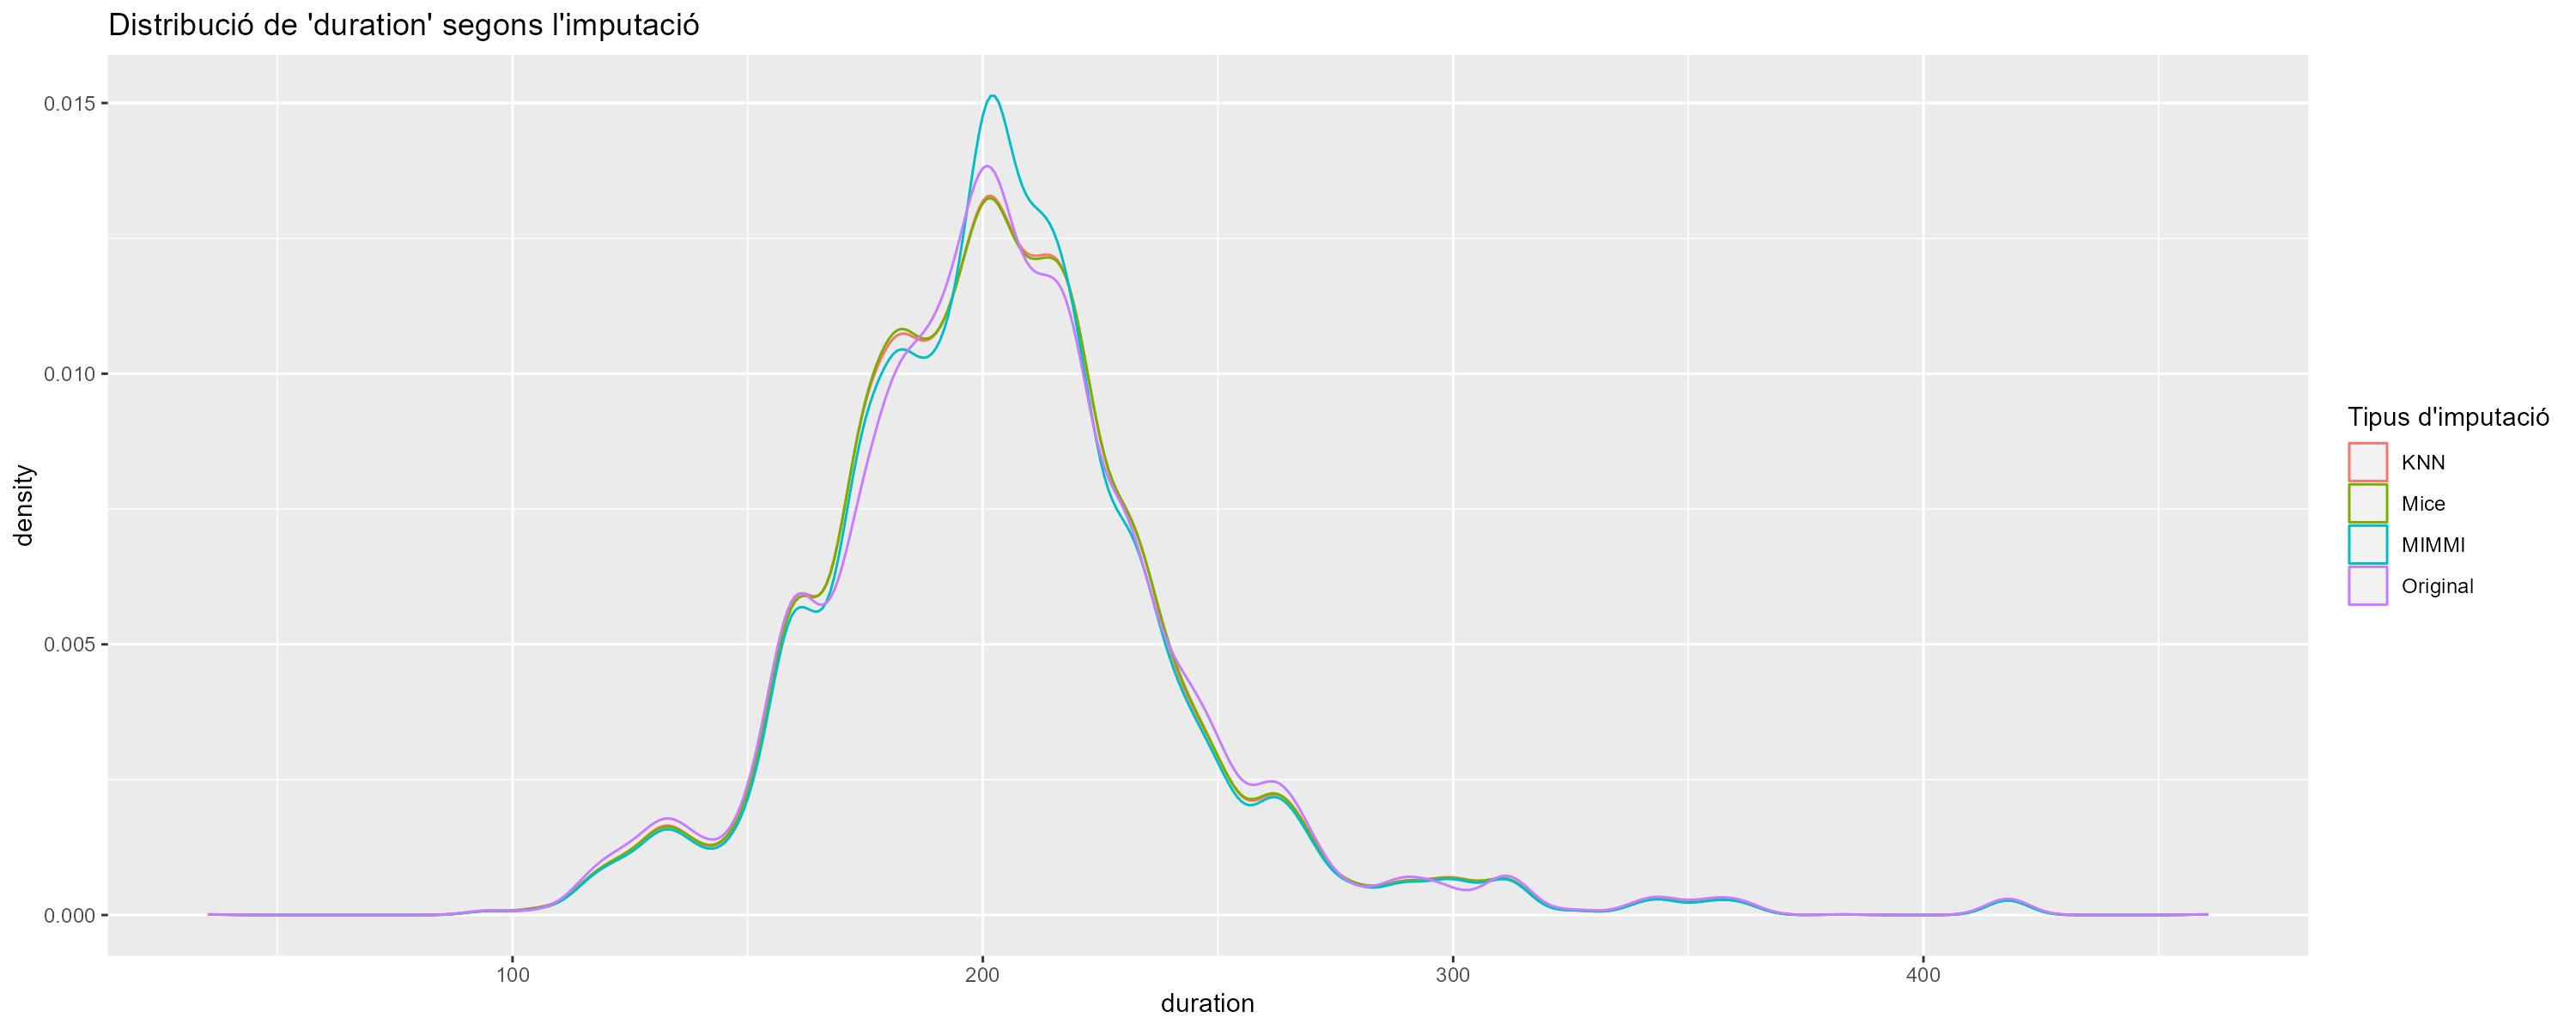
\includegraphics[width=0.8\textwidth]{Images/3_Preprocessing/distrib_imputation_duration.png}
    \caption{Distribucions de duration després de la imputació}
    \label{fig:Preprocessing_distribduration}
\end{figure}

\begin{figure}[H]
    \centering
    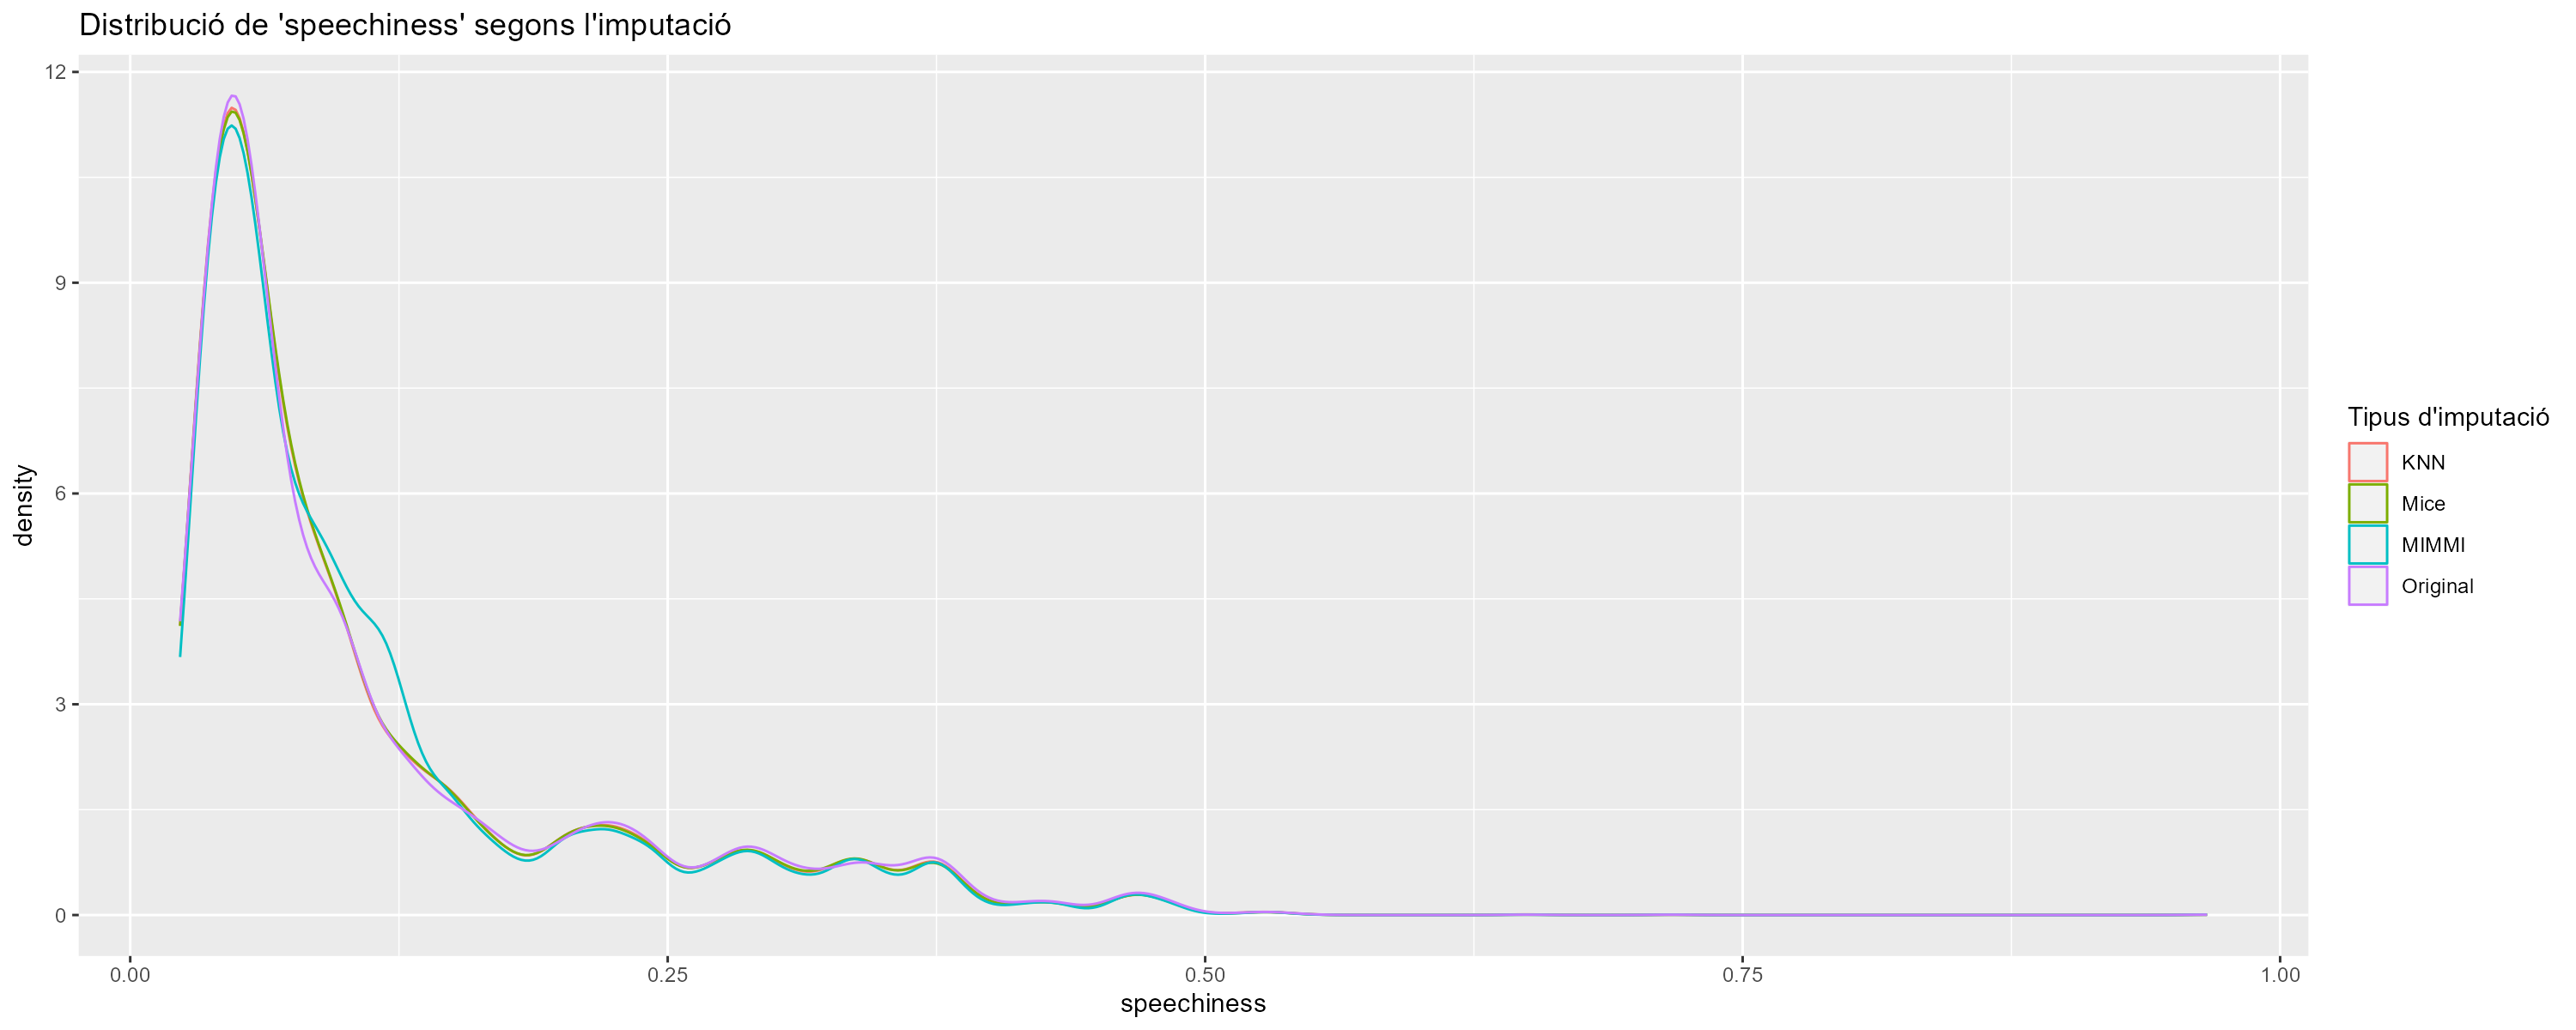
\includegraphics[width=0.8\textwidth]{Images/3_Preprocessing/distrib_imputation_speechiness.png}
    \caption{Distribucions de speechiness després de la imputació}
    \label{fig:Preprocessing_distribspeech}
\end{figure}

A partir d'aquestes distribucions, observem com el MICE i el KNN són els que han donat resultats millors, i que s'apropen més a la distribució real. D'altra banda, el MIMMI té alguns pics en les mitjanes dels clústers que ha fet servir per imputar. Després de valorar les opcions, hem decidit usar les dades imputades usant KNN.

Addicionalment, algunes de les altres distribucions també s'han arreglat. Per exemple, track\_name, aquest cop sí que és la distribució real (ja que en l'anàlisi anterior, algunes cançons contenien missing i s'havia ignorat aquella fila). En aquest cas, queda com la figura figura \ref{fig:UnivariateP_track}. A més, per exemple \textit{gender} ara té la categoria \textit{Unknown}, enlloc de \textit{na} (figura \ref{fig:UnivariateP_gender}).

\begin{figure}[H]
\centering
    \begin{minipage}{.4\textwidth}
        \centering
        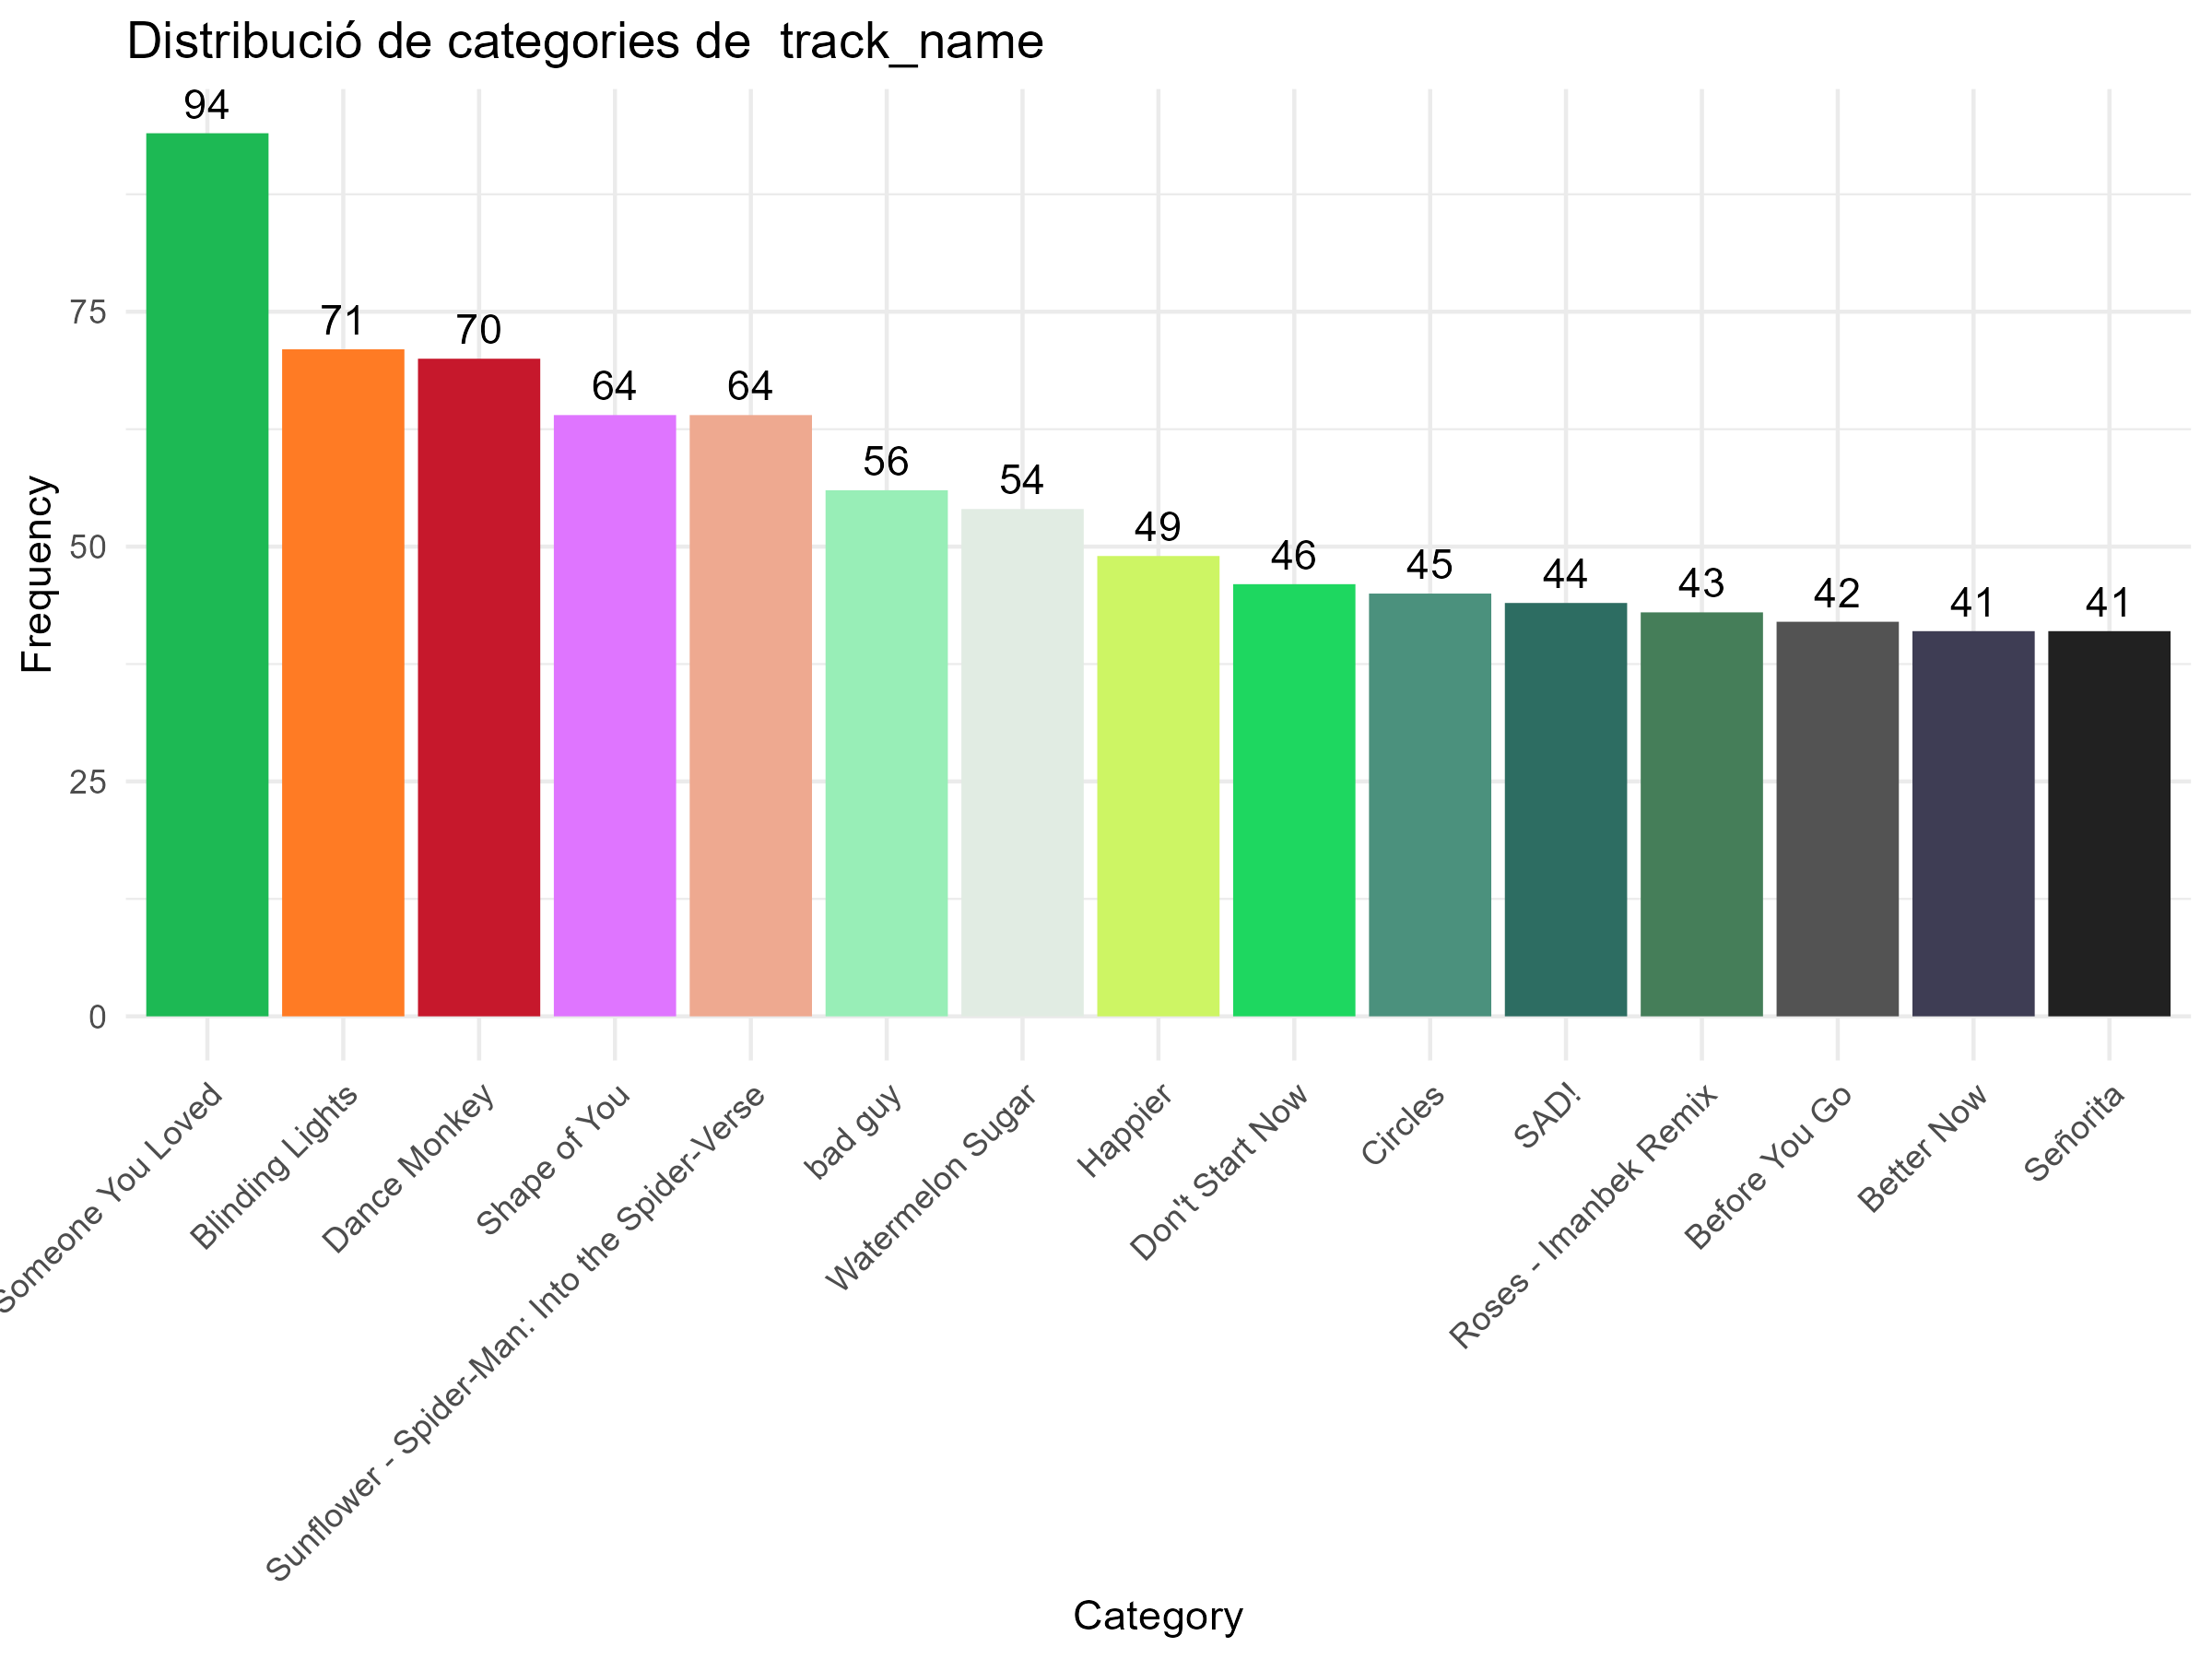
\includegraphics[width=0.95\linewidth]{Images/3_Preprocessing/bar_track_name.png}
        \caption{Bar plot de \textit{track\_name}}
        \label{fig:UnivariateP_track}
    \end{minipage}%
    \begin{minipage}{.4\textwidth}
        \centering
        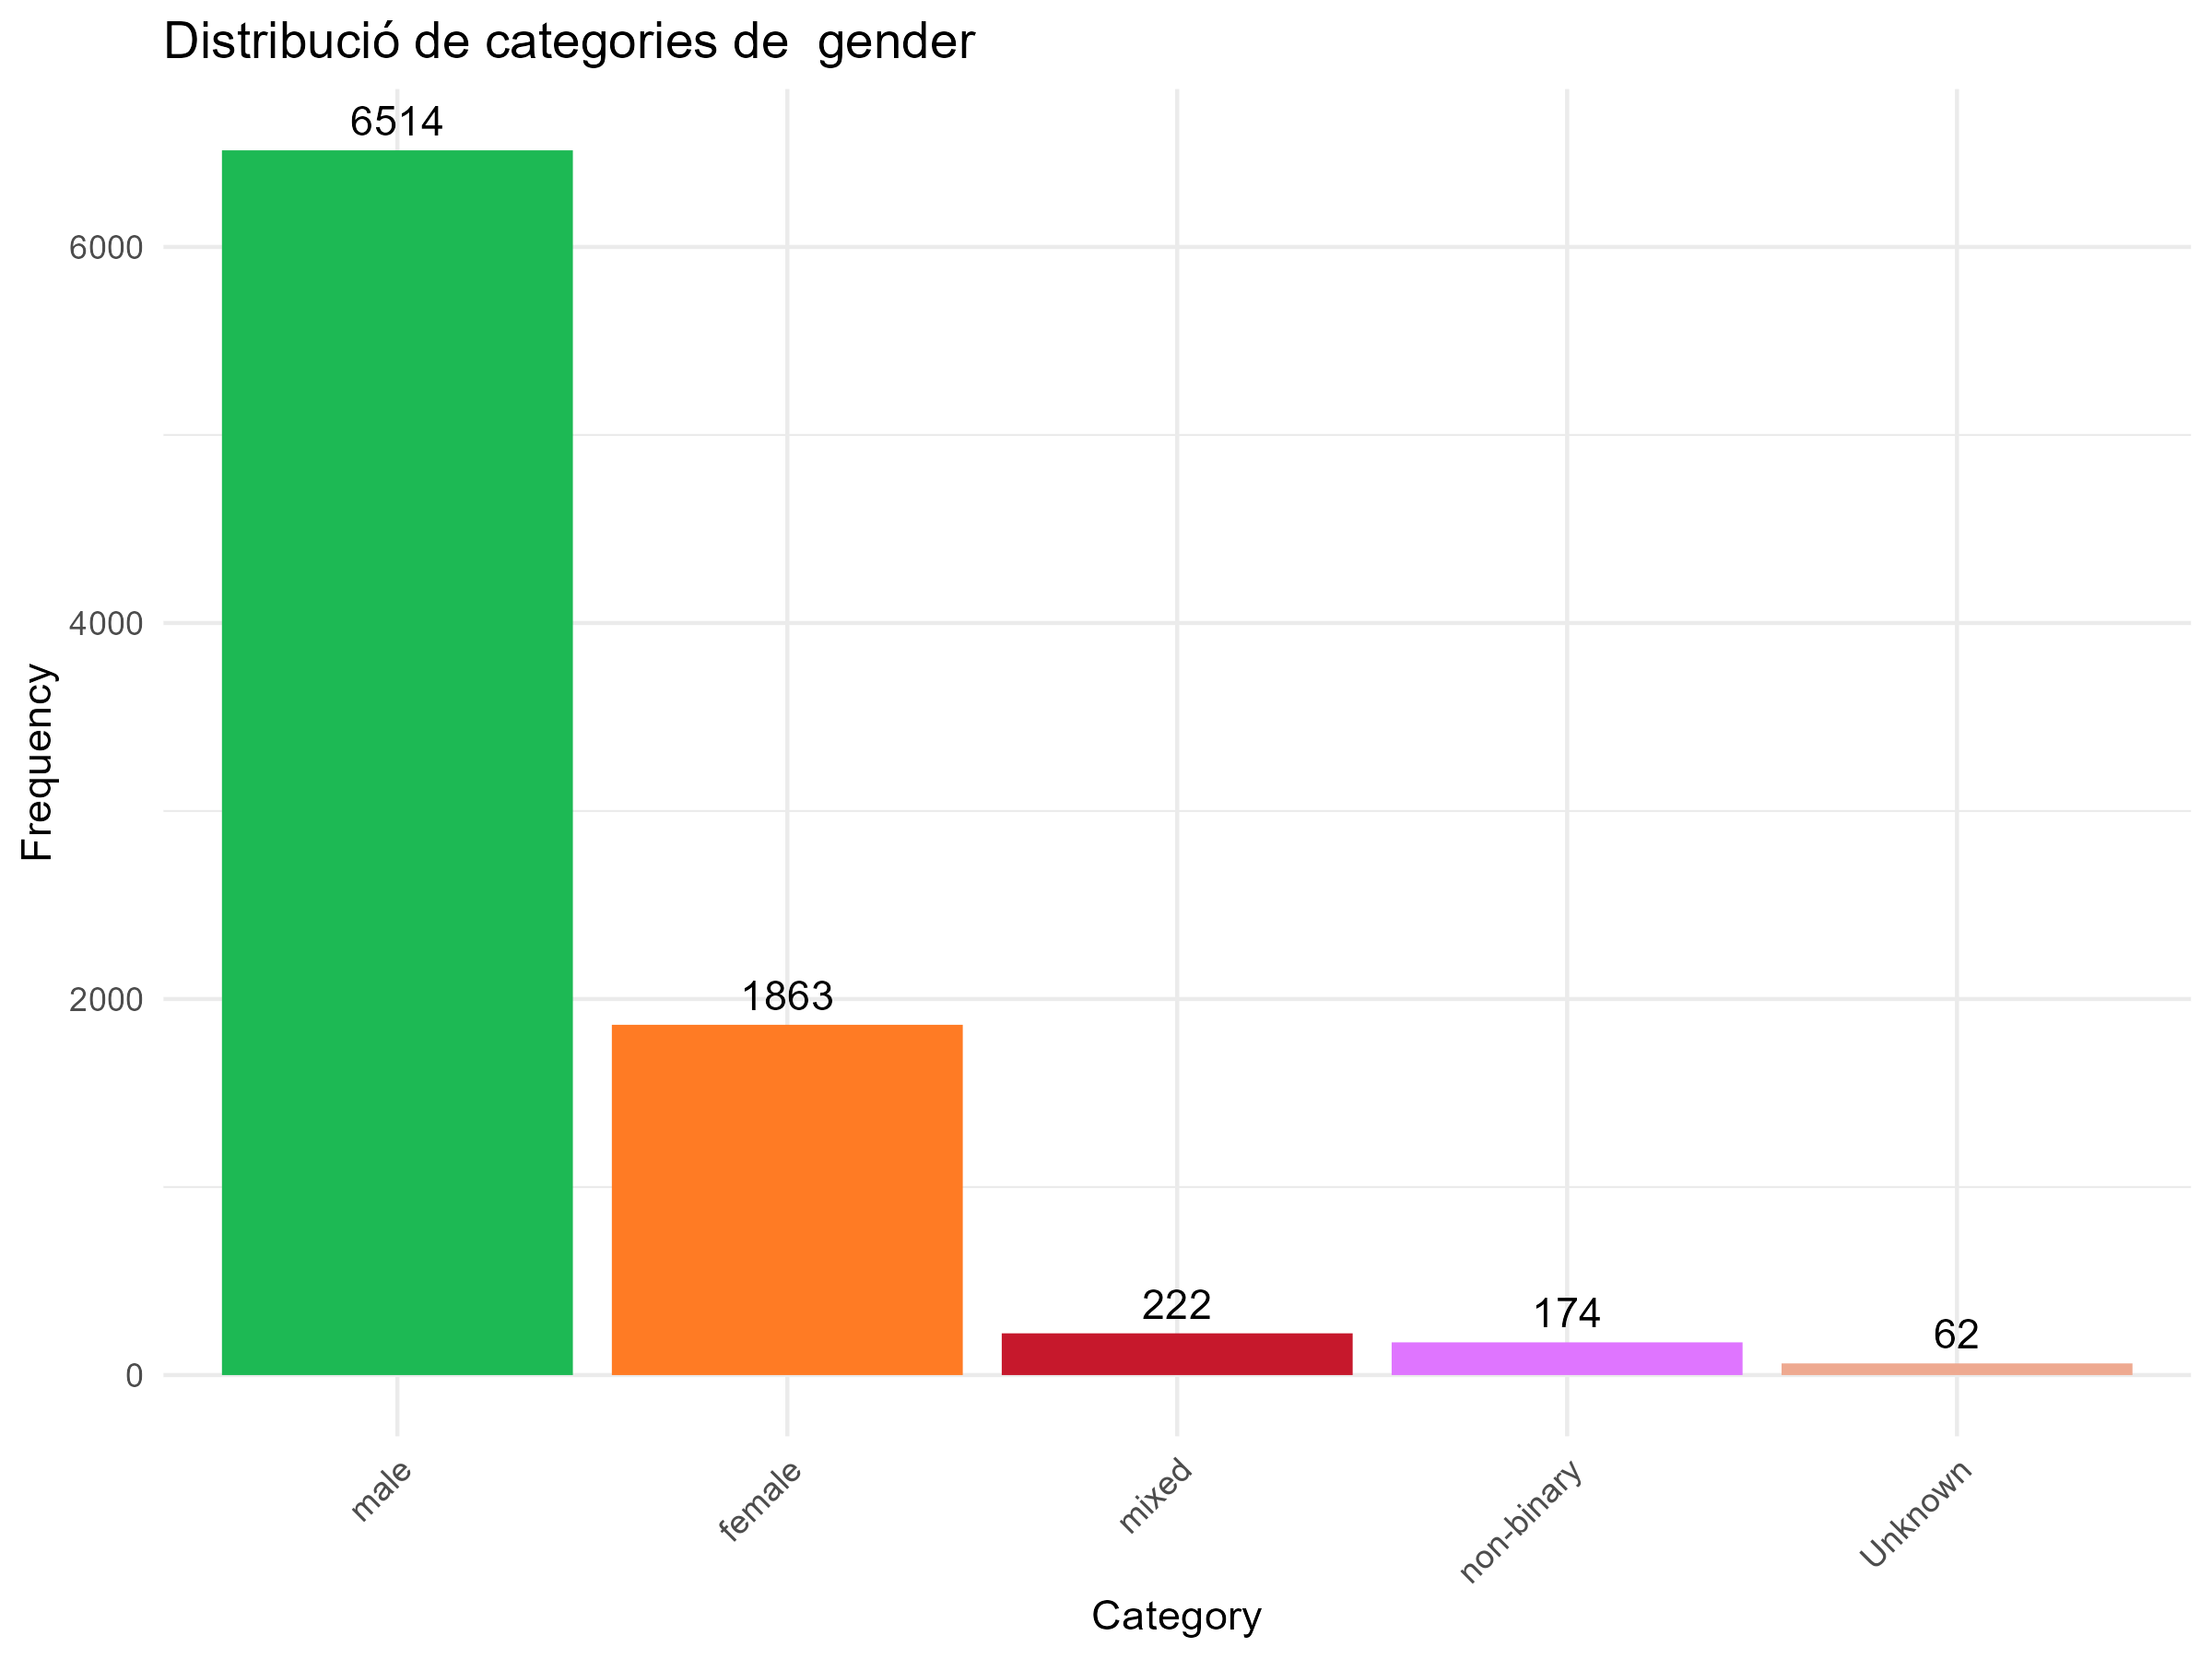
\includegraphics[width=0.95\linewidth]{Images/3_Preprocessing/bar_gender.png}
        \caption{Bar plot de \textit{gender}}
        \label{fig:UnivariateP_gender}
    \end{minipage}%
\end{figure}

Degut a la naturalesa de la base de dades, era possible realitzar un altre anàlisi descriptiu de dades: separant per artistes únics (300 instàncies), i separant per cançons úniques (1019). D'aquesta manera, podem saber per exemple realment quants artistes són de cada ciutat o país (enlloc de quants cops apareix un artista d'aquell lloc) (figura \ref{fig:UnivariateP_a_city}). L'ordre de les ciutats ha canviat, situant-se en aquest cas Washington D.C. en el segon lloc per davant de San Juan (capital de Puerto Rico). També hi ha alguna numèrica que canvia, com artist followers que en aquest cas té una distribució més suavitzada (sense els pics que tenia si no tenim en compte artistes únics) (figura \ref{fig:UnivariateP_a_followers}).

\begin{figure}[H]
\centering
    \begin{minipage}{.4\textwidth}
        \centering
        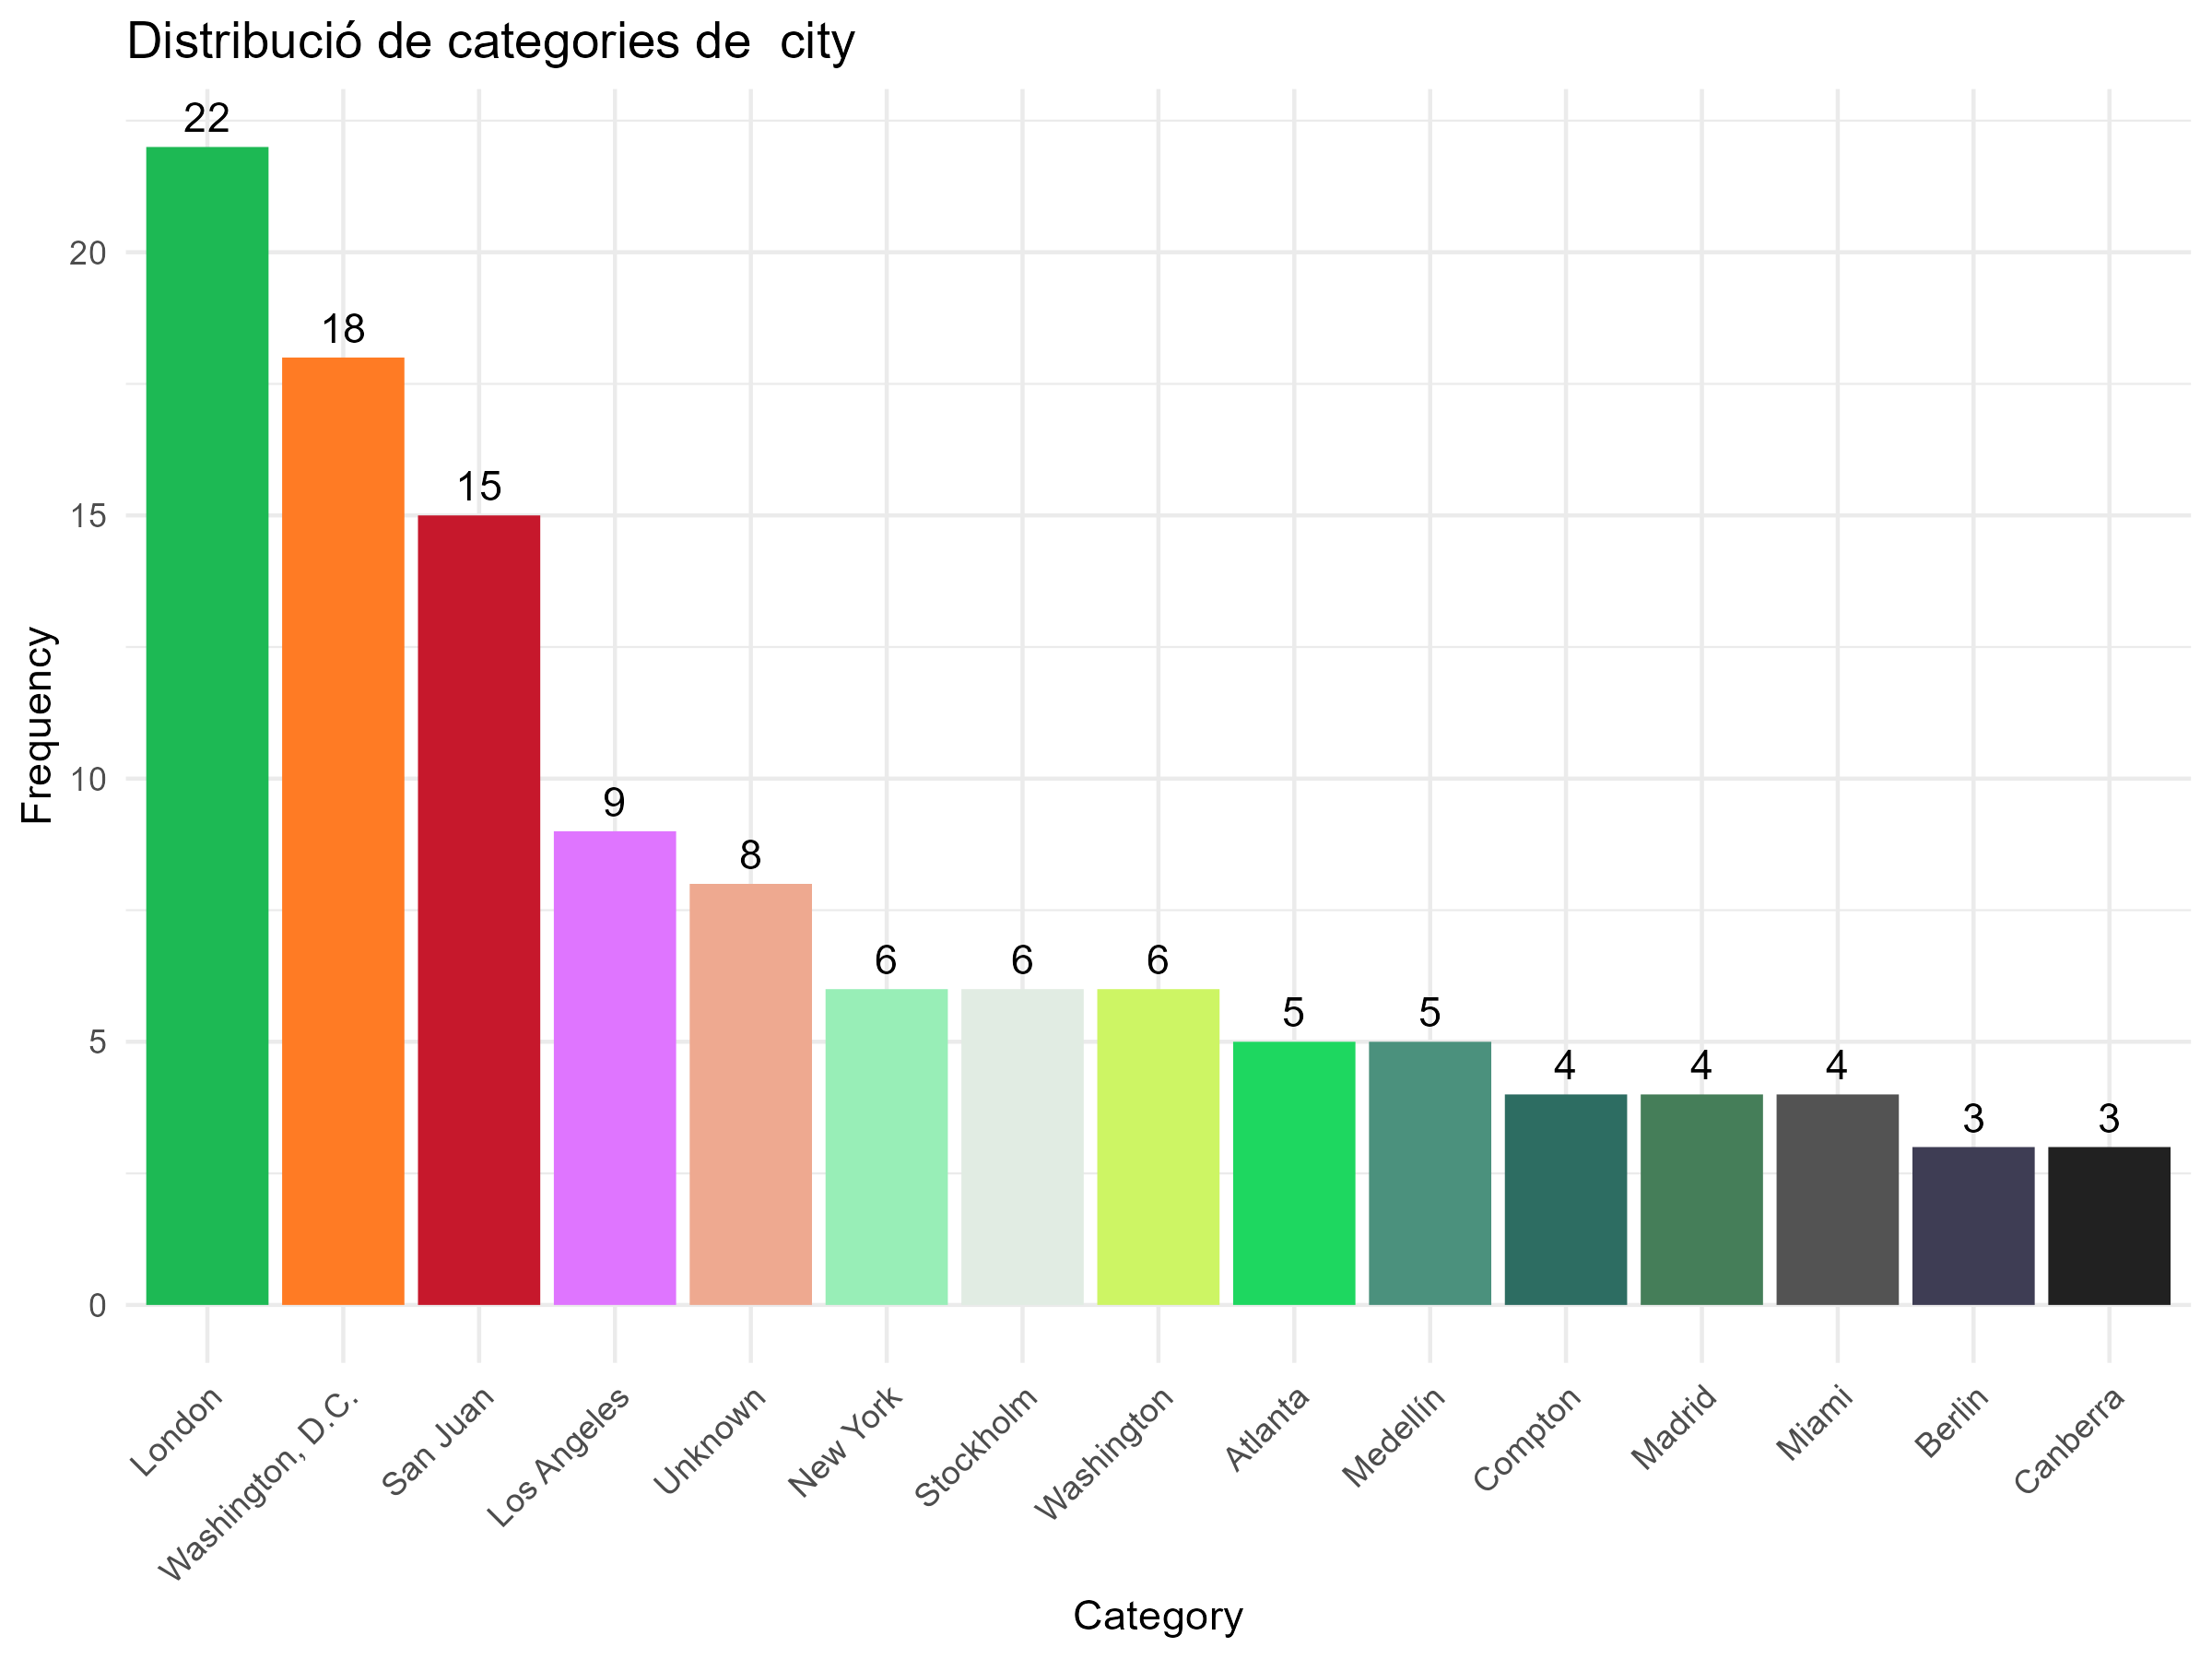
\includegraphics[width=0.95\linewidth]{Images/3_Preprocessing/Artist/bar_city.png}
        \caption{Bar plot de \textit{city} per artistes únics}
        \label{fig:UnivariateP_a_city}
    \end{minipage}%
    \begin{minipage}{.4\textwidth}
        \centering
        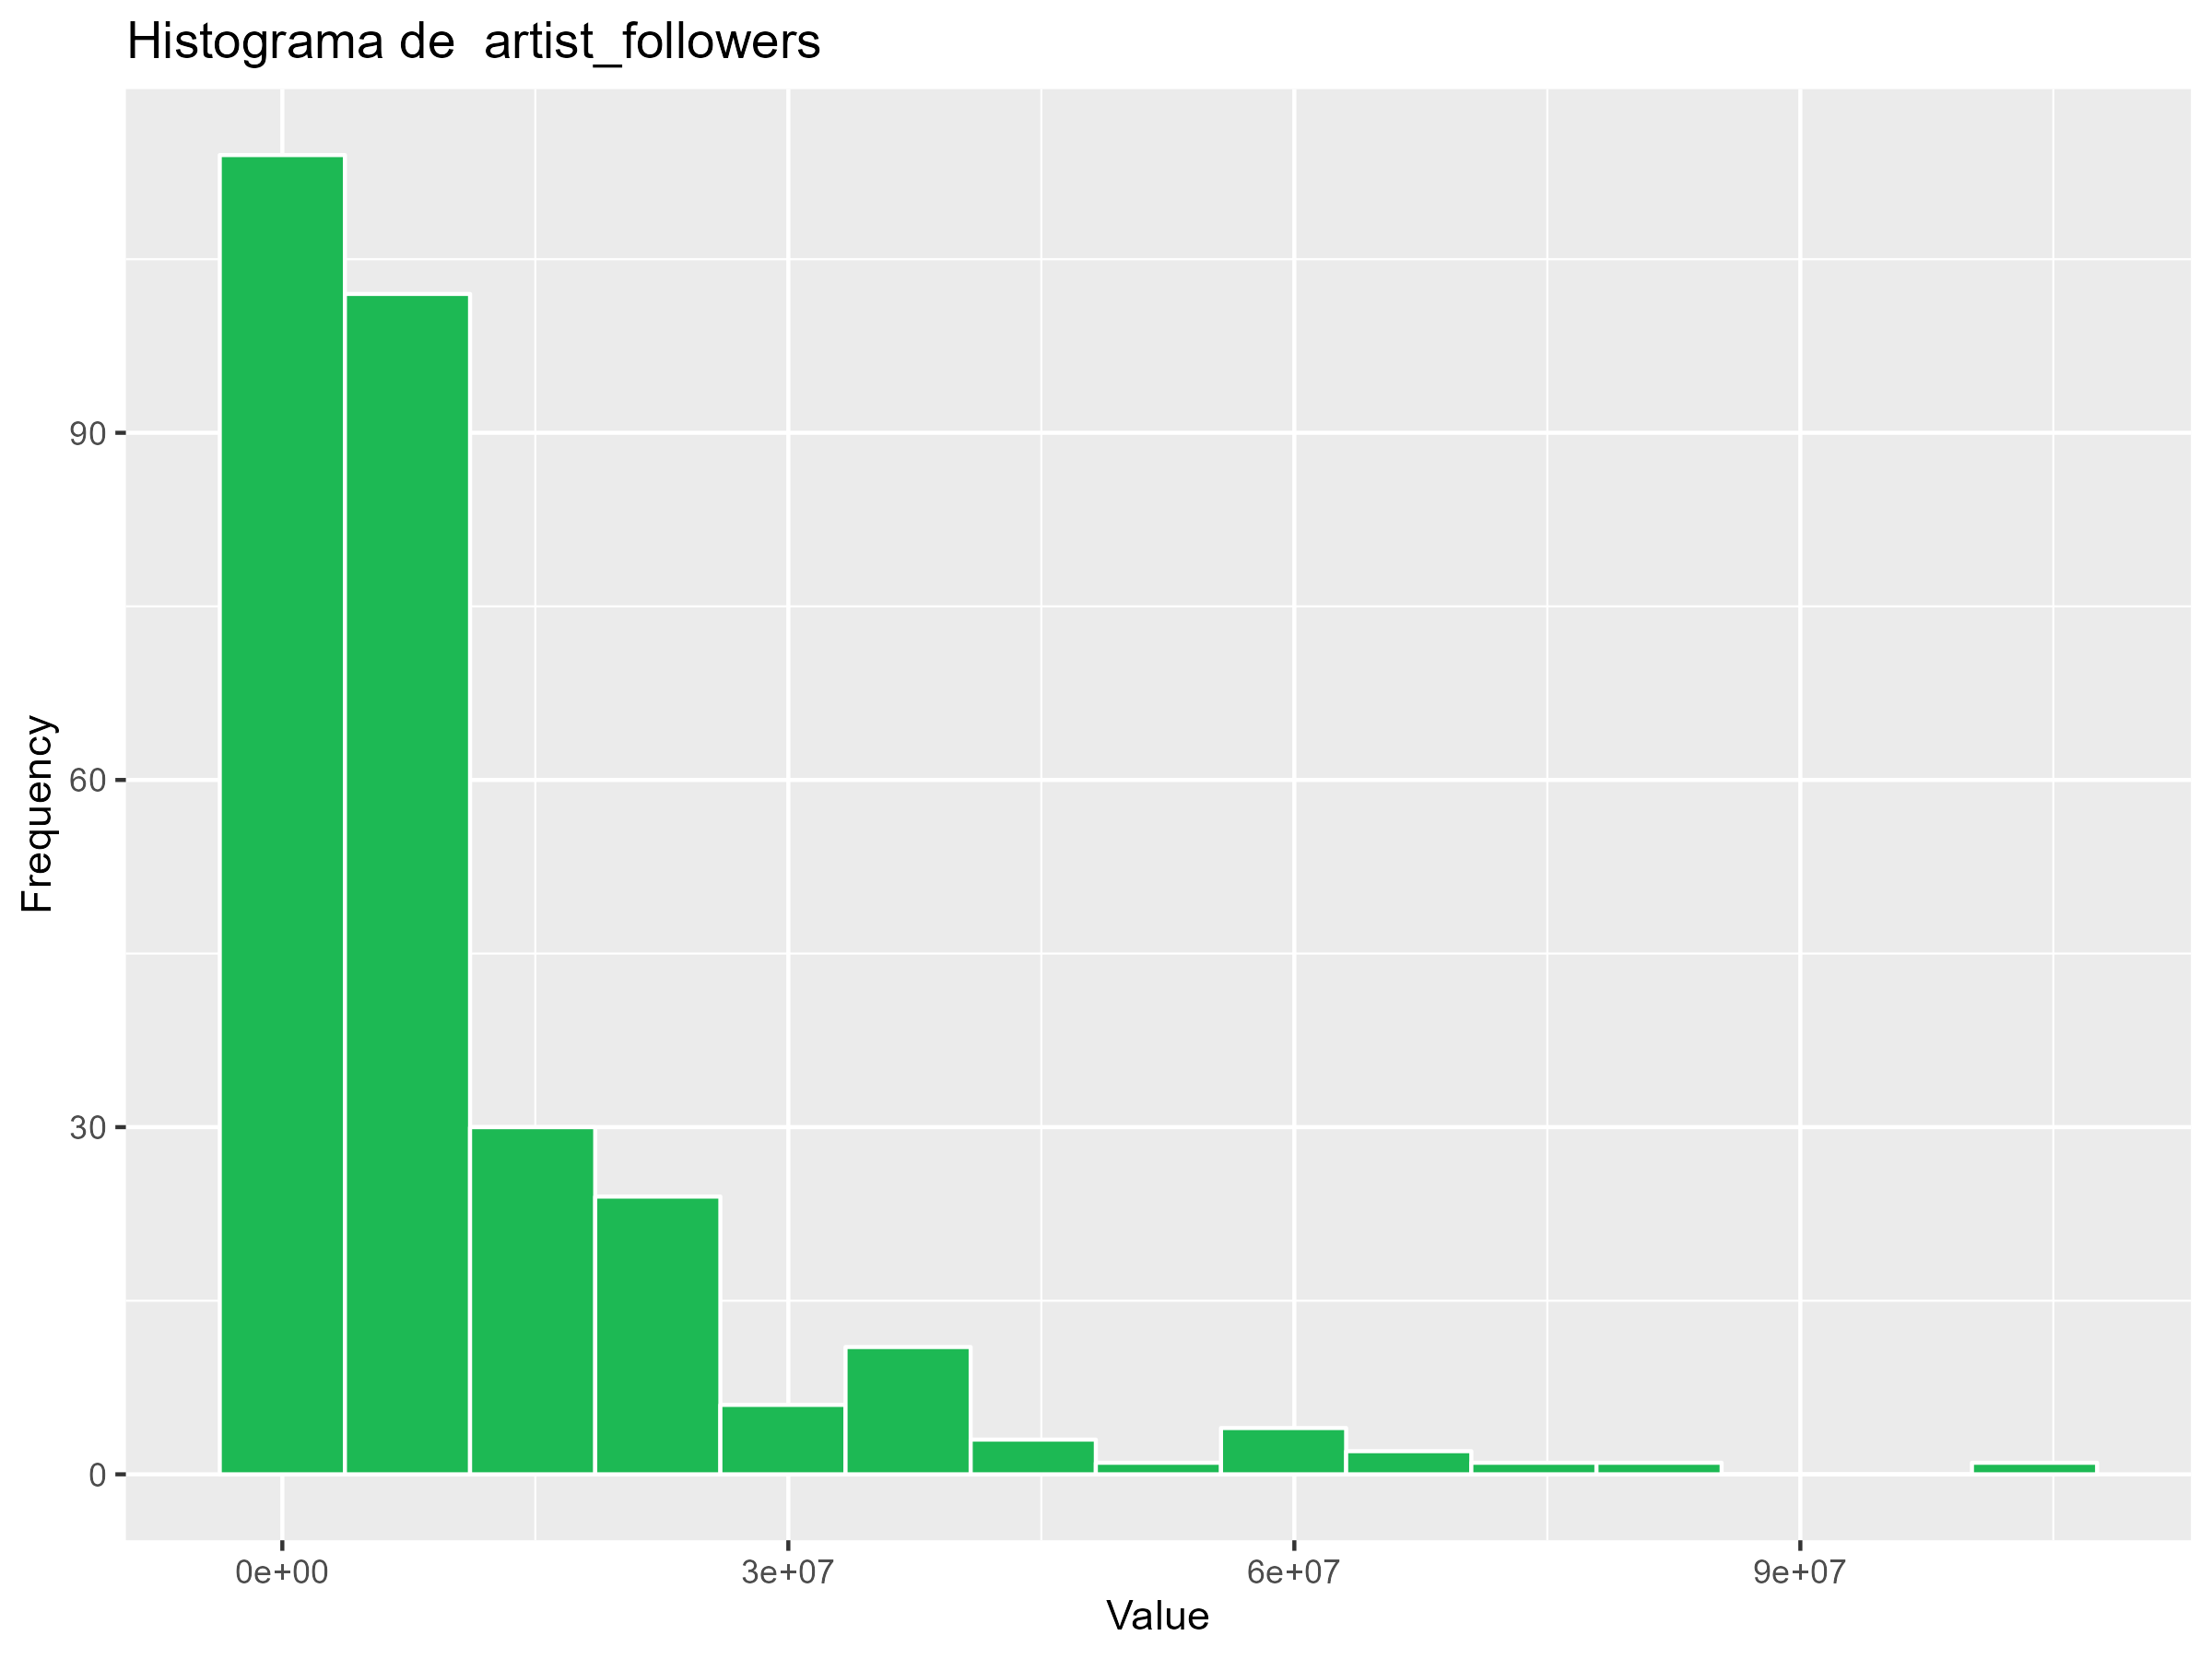
\includegraphics[width=0.95\linewidth]{Images/3_Preprocessing/Artist/hist_artist_followers.png}
        \caption{Histograma de \textit{artist followers} per artistes únics}
        \label{fig:UnivariateP_a_followers}
    \end{minipage}%
\end{figure}


El mateix podem fer separant per cançó única. Moltes de les distribucions segueixen sent iguals, però per exemple collab passa a tenir menys percentatge de valors TRUE (indicant que les col·laboracions tenen tendència a aparèixer durant més setmanes en el top) (figura \ref{fig:UnivariateP_t_collab}). També hi ha un percentatge menor de cançons Pop, com es pot veure a la figura figura \ref{fig:UnivariateP_t_pop}.

\begin{figure}[H]
\centering
    \begin{minipage}{.4\textwidth}
        \centering
        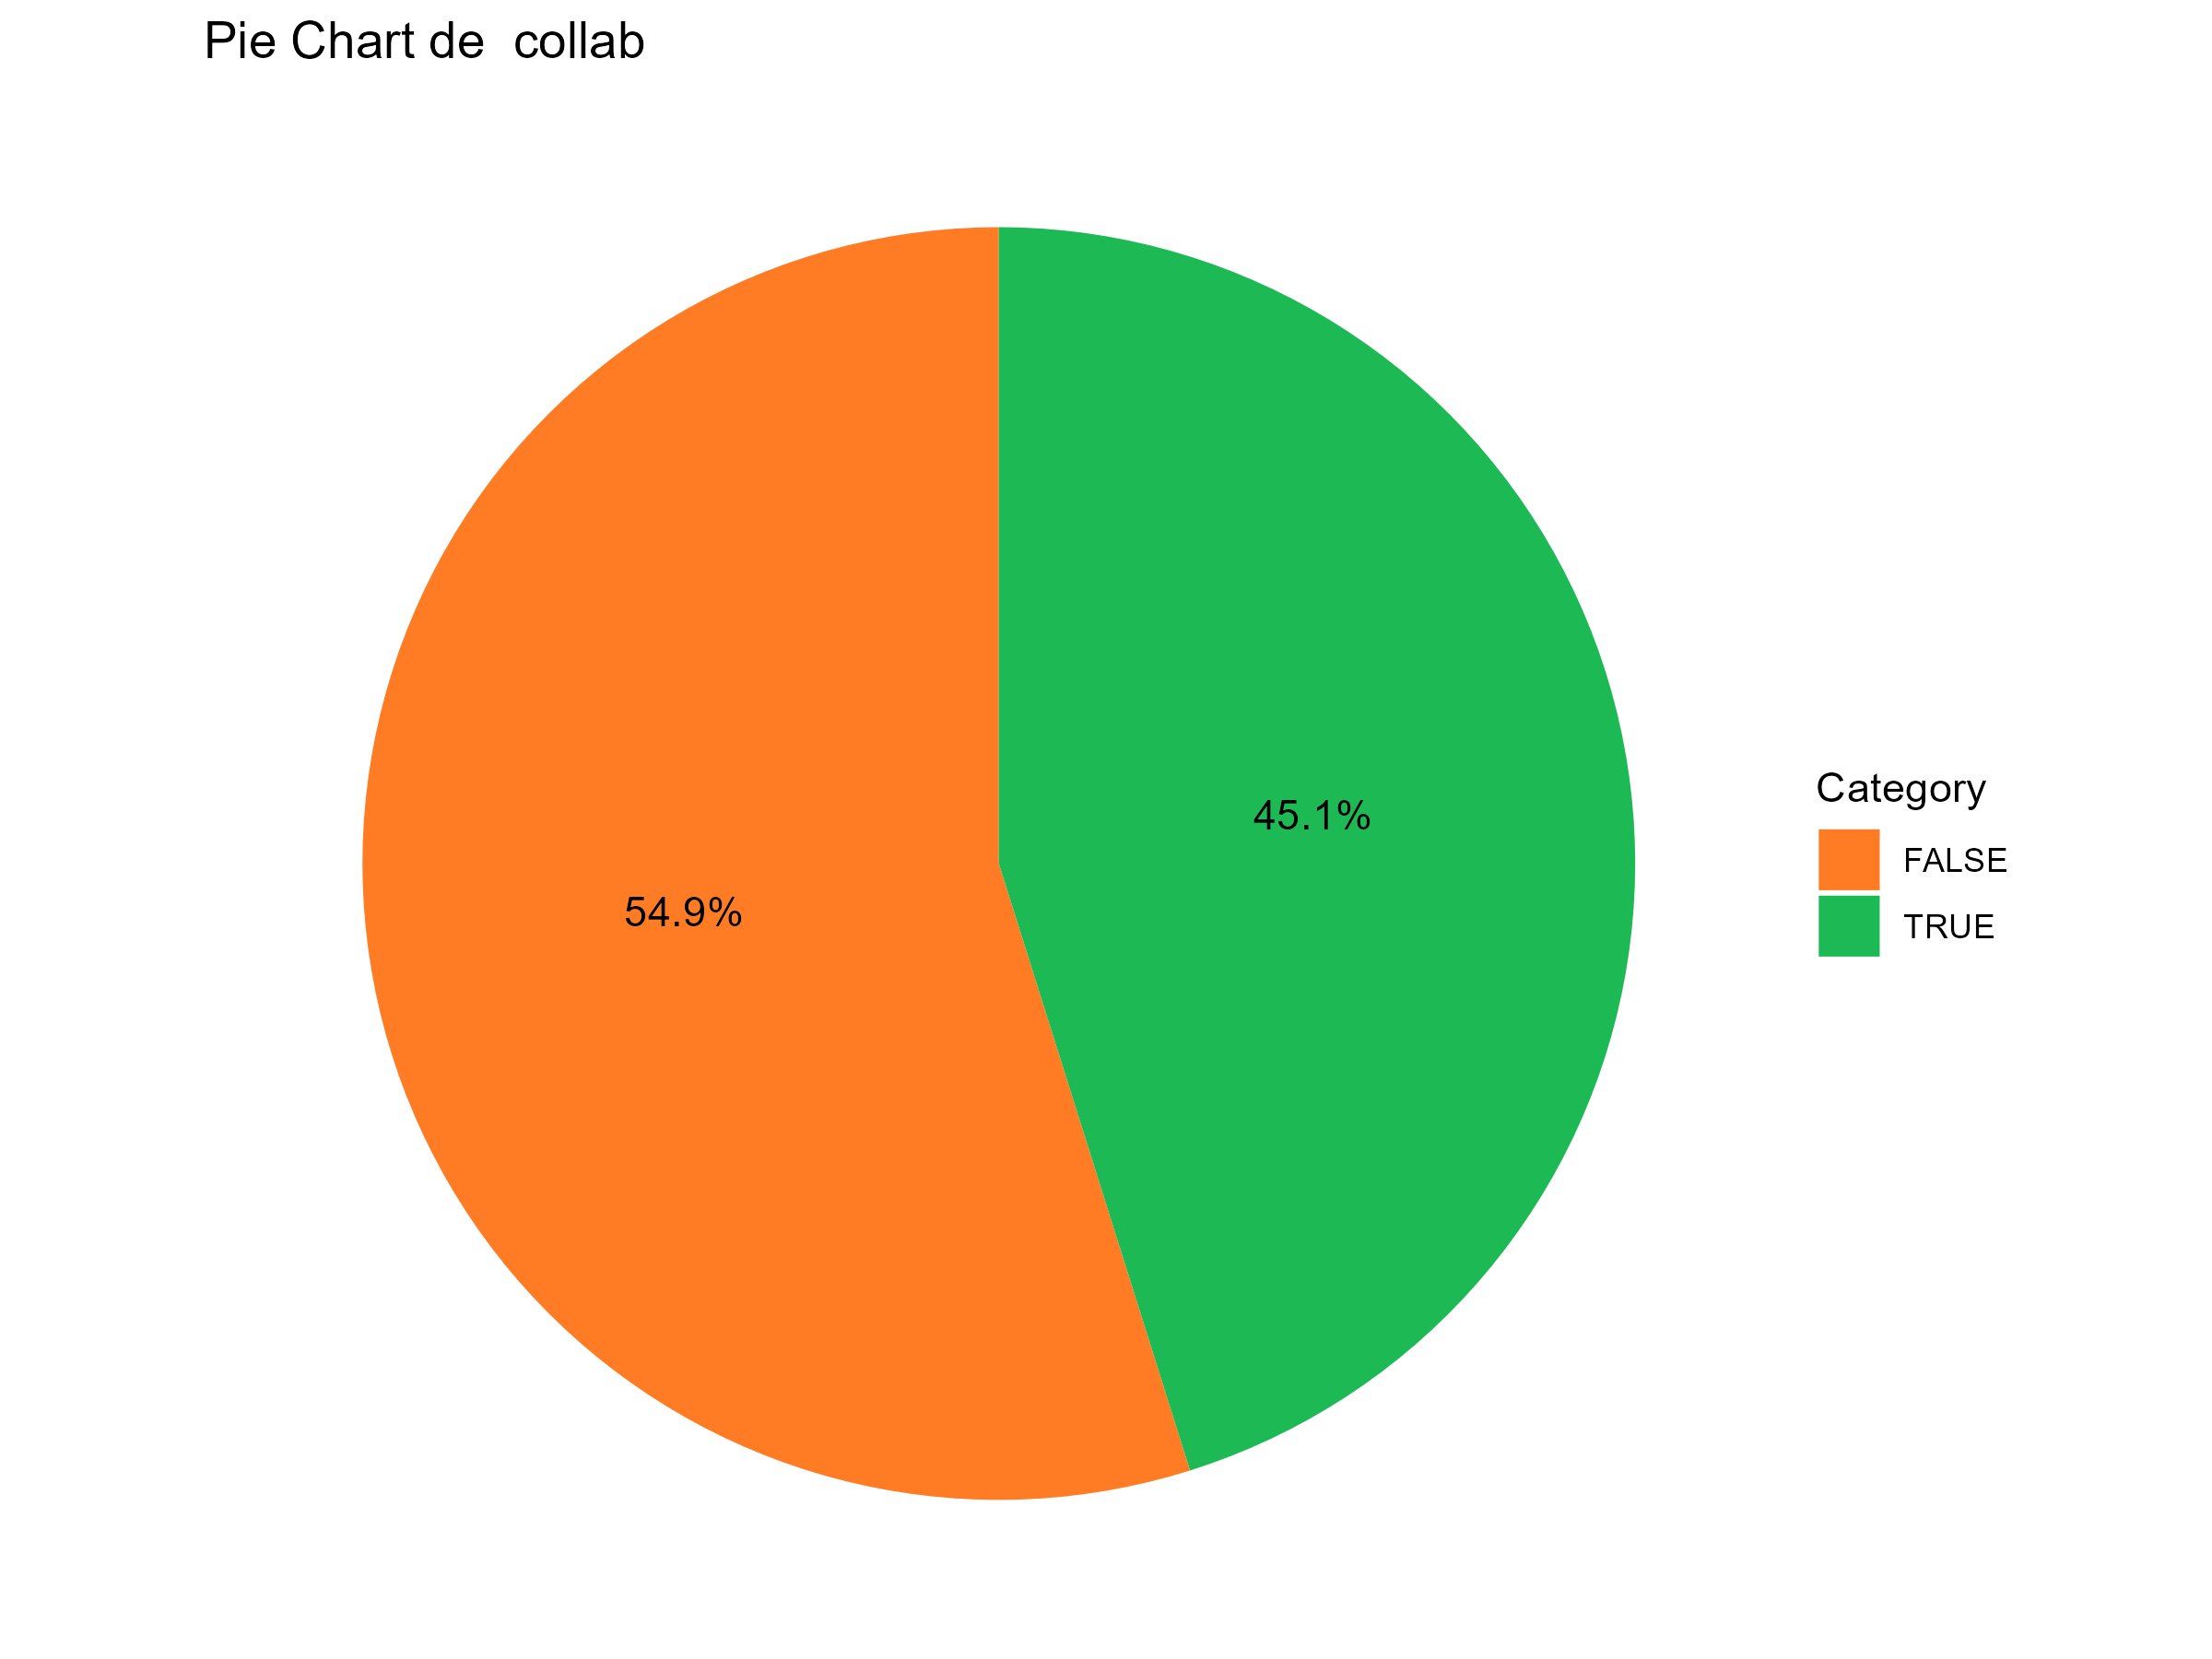
\includegraphics[width=0.95\linewidth]{Images/3_Preprocessing/Track/pie_collab.png}
        \caption{Pie chart de \textit{collab} per cançons úniques}
        \label{fig:UnivariateP_t_collab}
    \end{minipage}%
    \begin{minipage}{.4\textwidth}
        \centering
        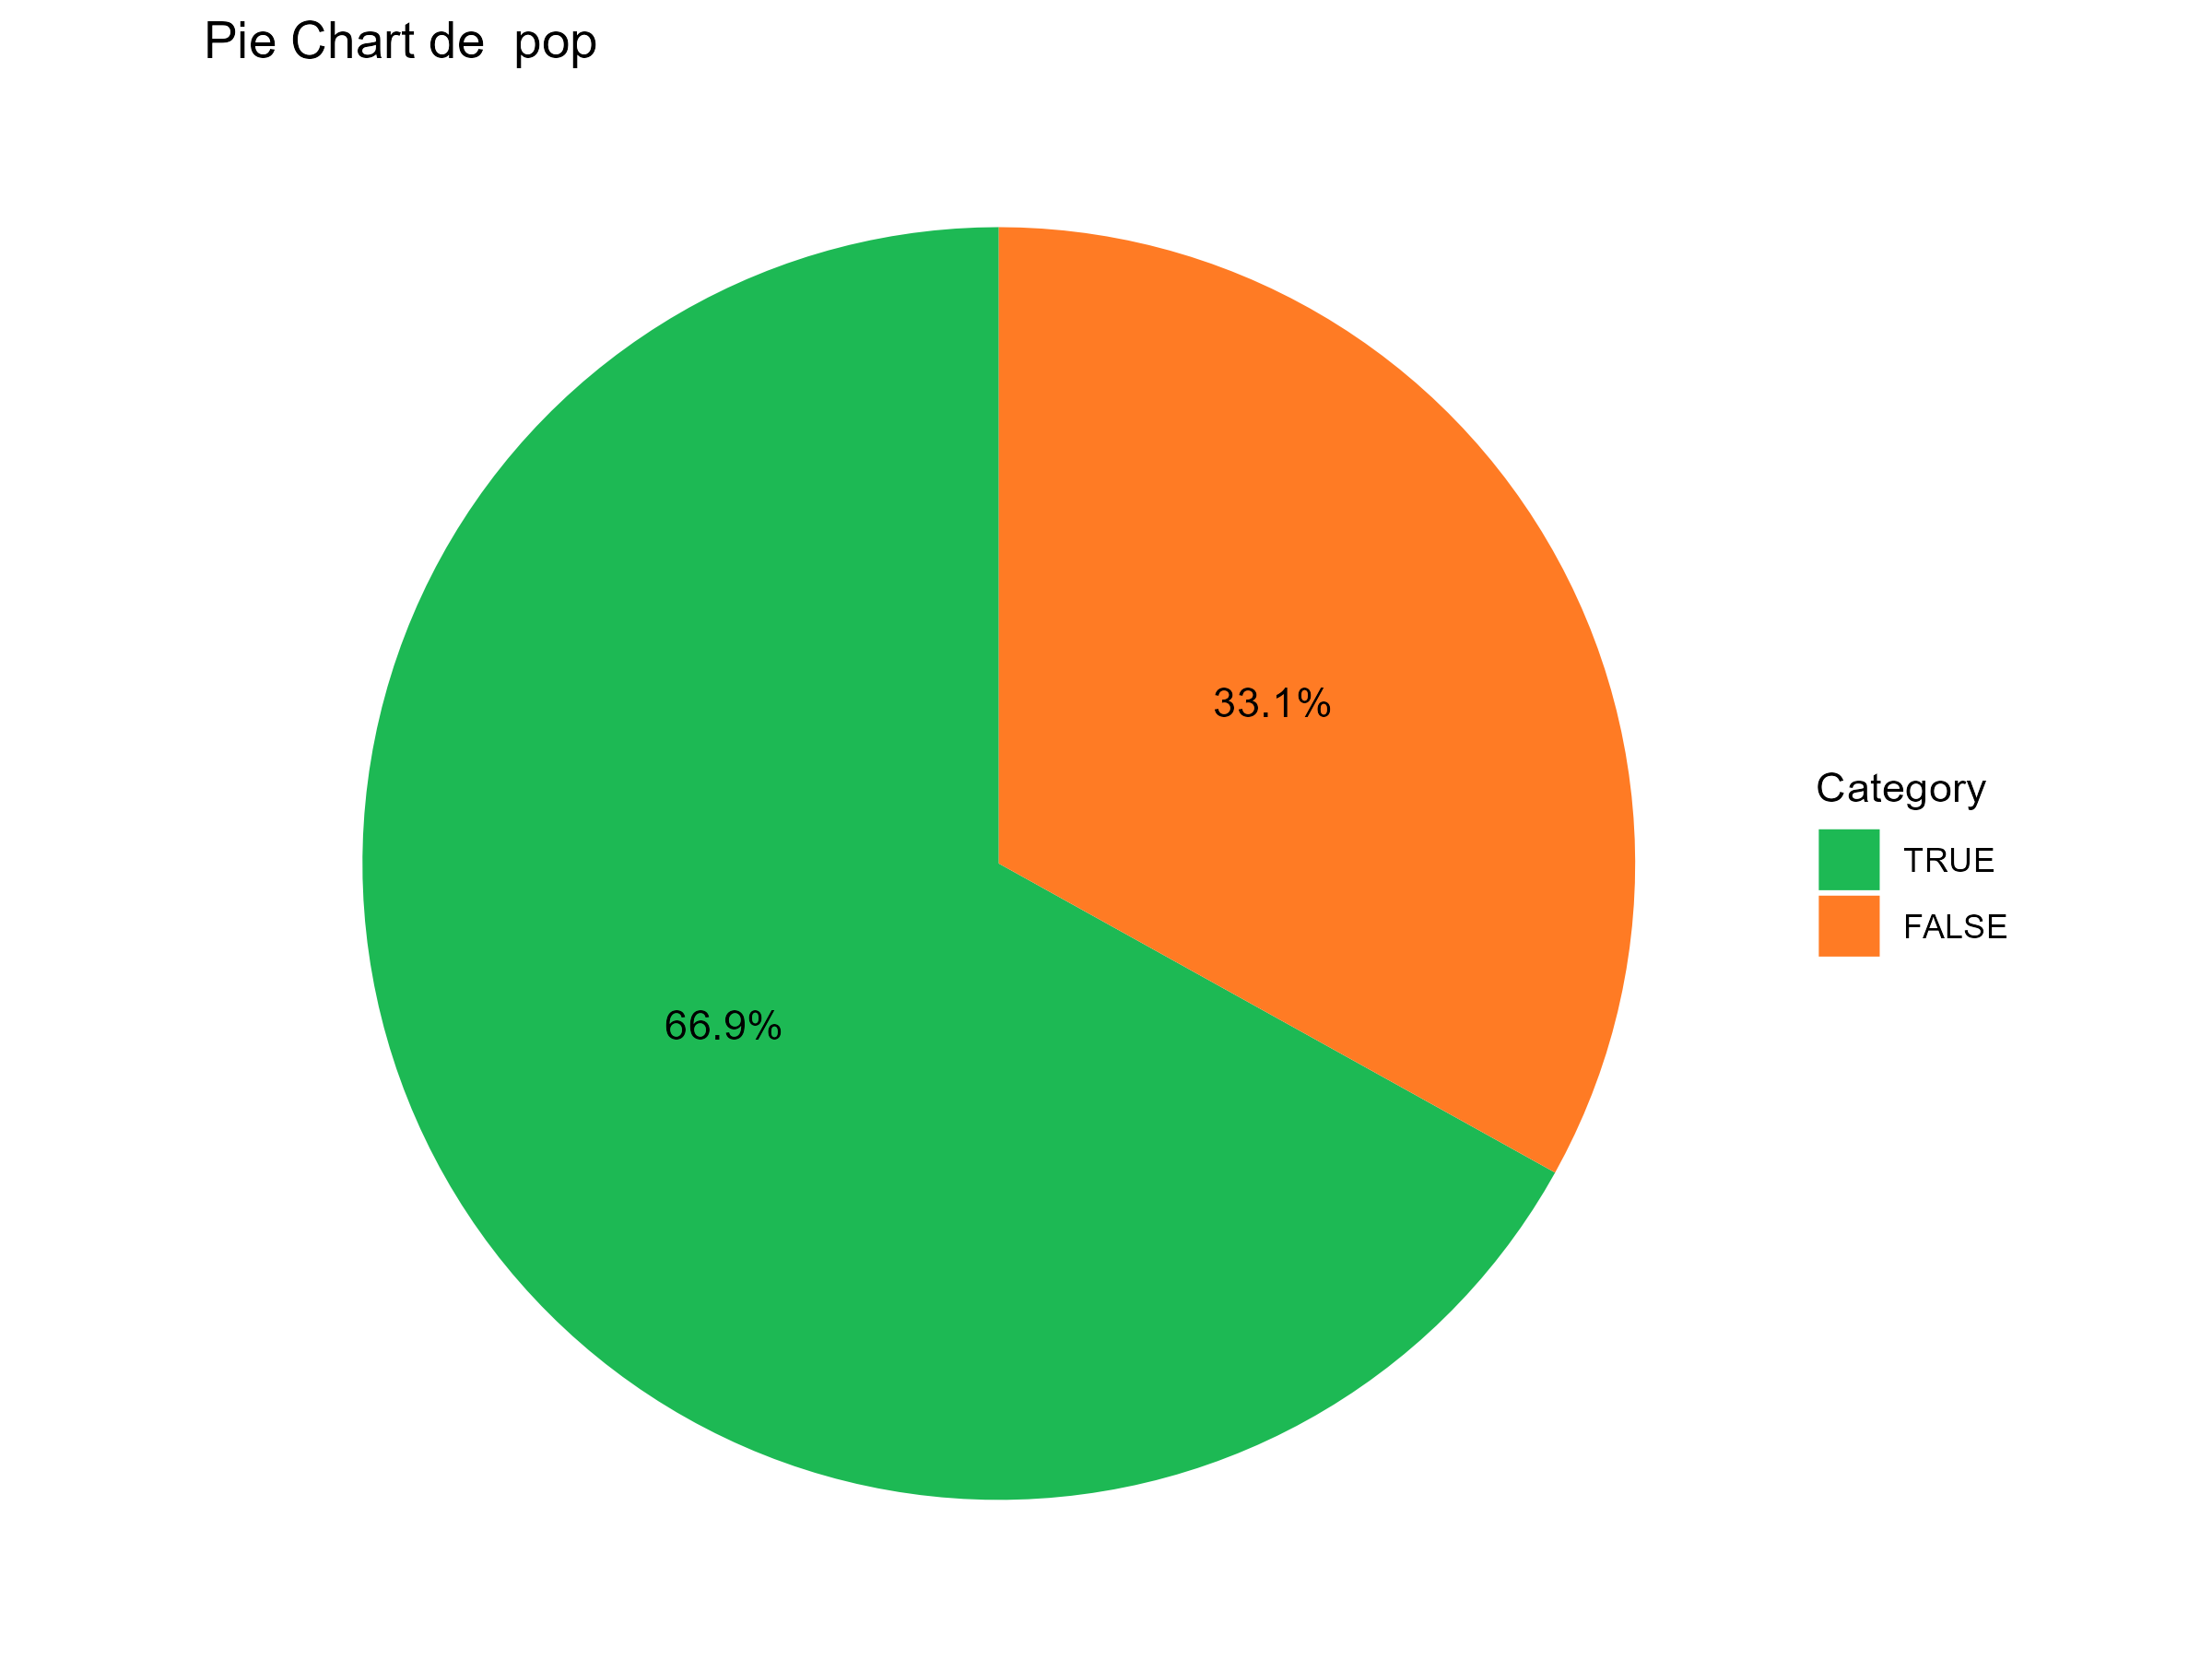
\includegraphics[width=0.95\linewidth]{Images/3_Preprocessing/Track/pie_pop.png}
        \caption{Pie chart de \textit{pop} per cançons úniques}
        \label{fig:UnivariateP_t_pop}
    \end{minipage}%
\end{figure}

També podem realitzar anàlisi bivariant que no haviem realitzat abans, amb les variables noves i correctes. Per exemple, es poden sumar el total de reproduccions (streams) per país i queda tal que \ref{fig:BivariateP_nationstreams} . Observem el predomini dels Estats Units en la indústria musical, seguit del Regne Unit, Canada i Puerto Rico. A més, podem analitzar també com influeix la nacionalitat en els gèneres, veient per exemple que el gènere latino prové sobretot d'artites de Puerto Rico, Colombia, i en menys mesura Espanya, Panama, Estats Units, República Dominicana i Venezuela (\ref{fig:BivariateP_nationlati}).

\begin{figure}[H]
\centering
    \begin{minipage}{.4\textwidth}
        \centering
        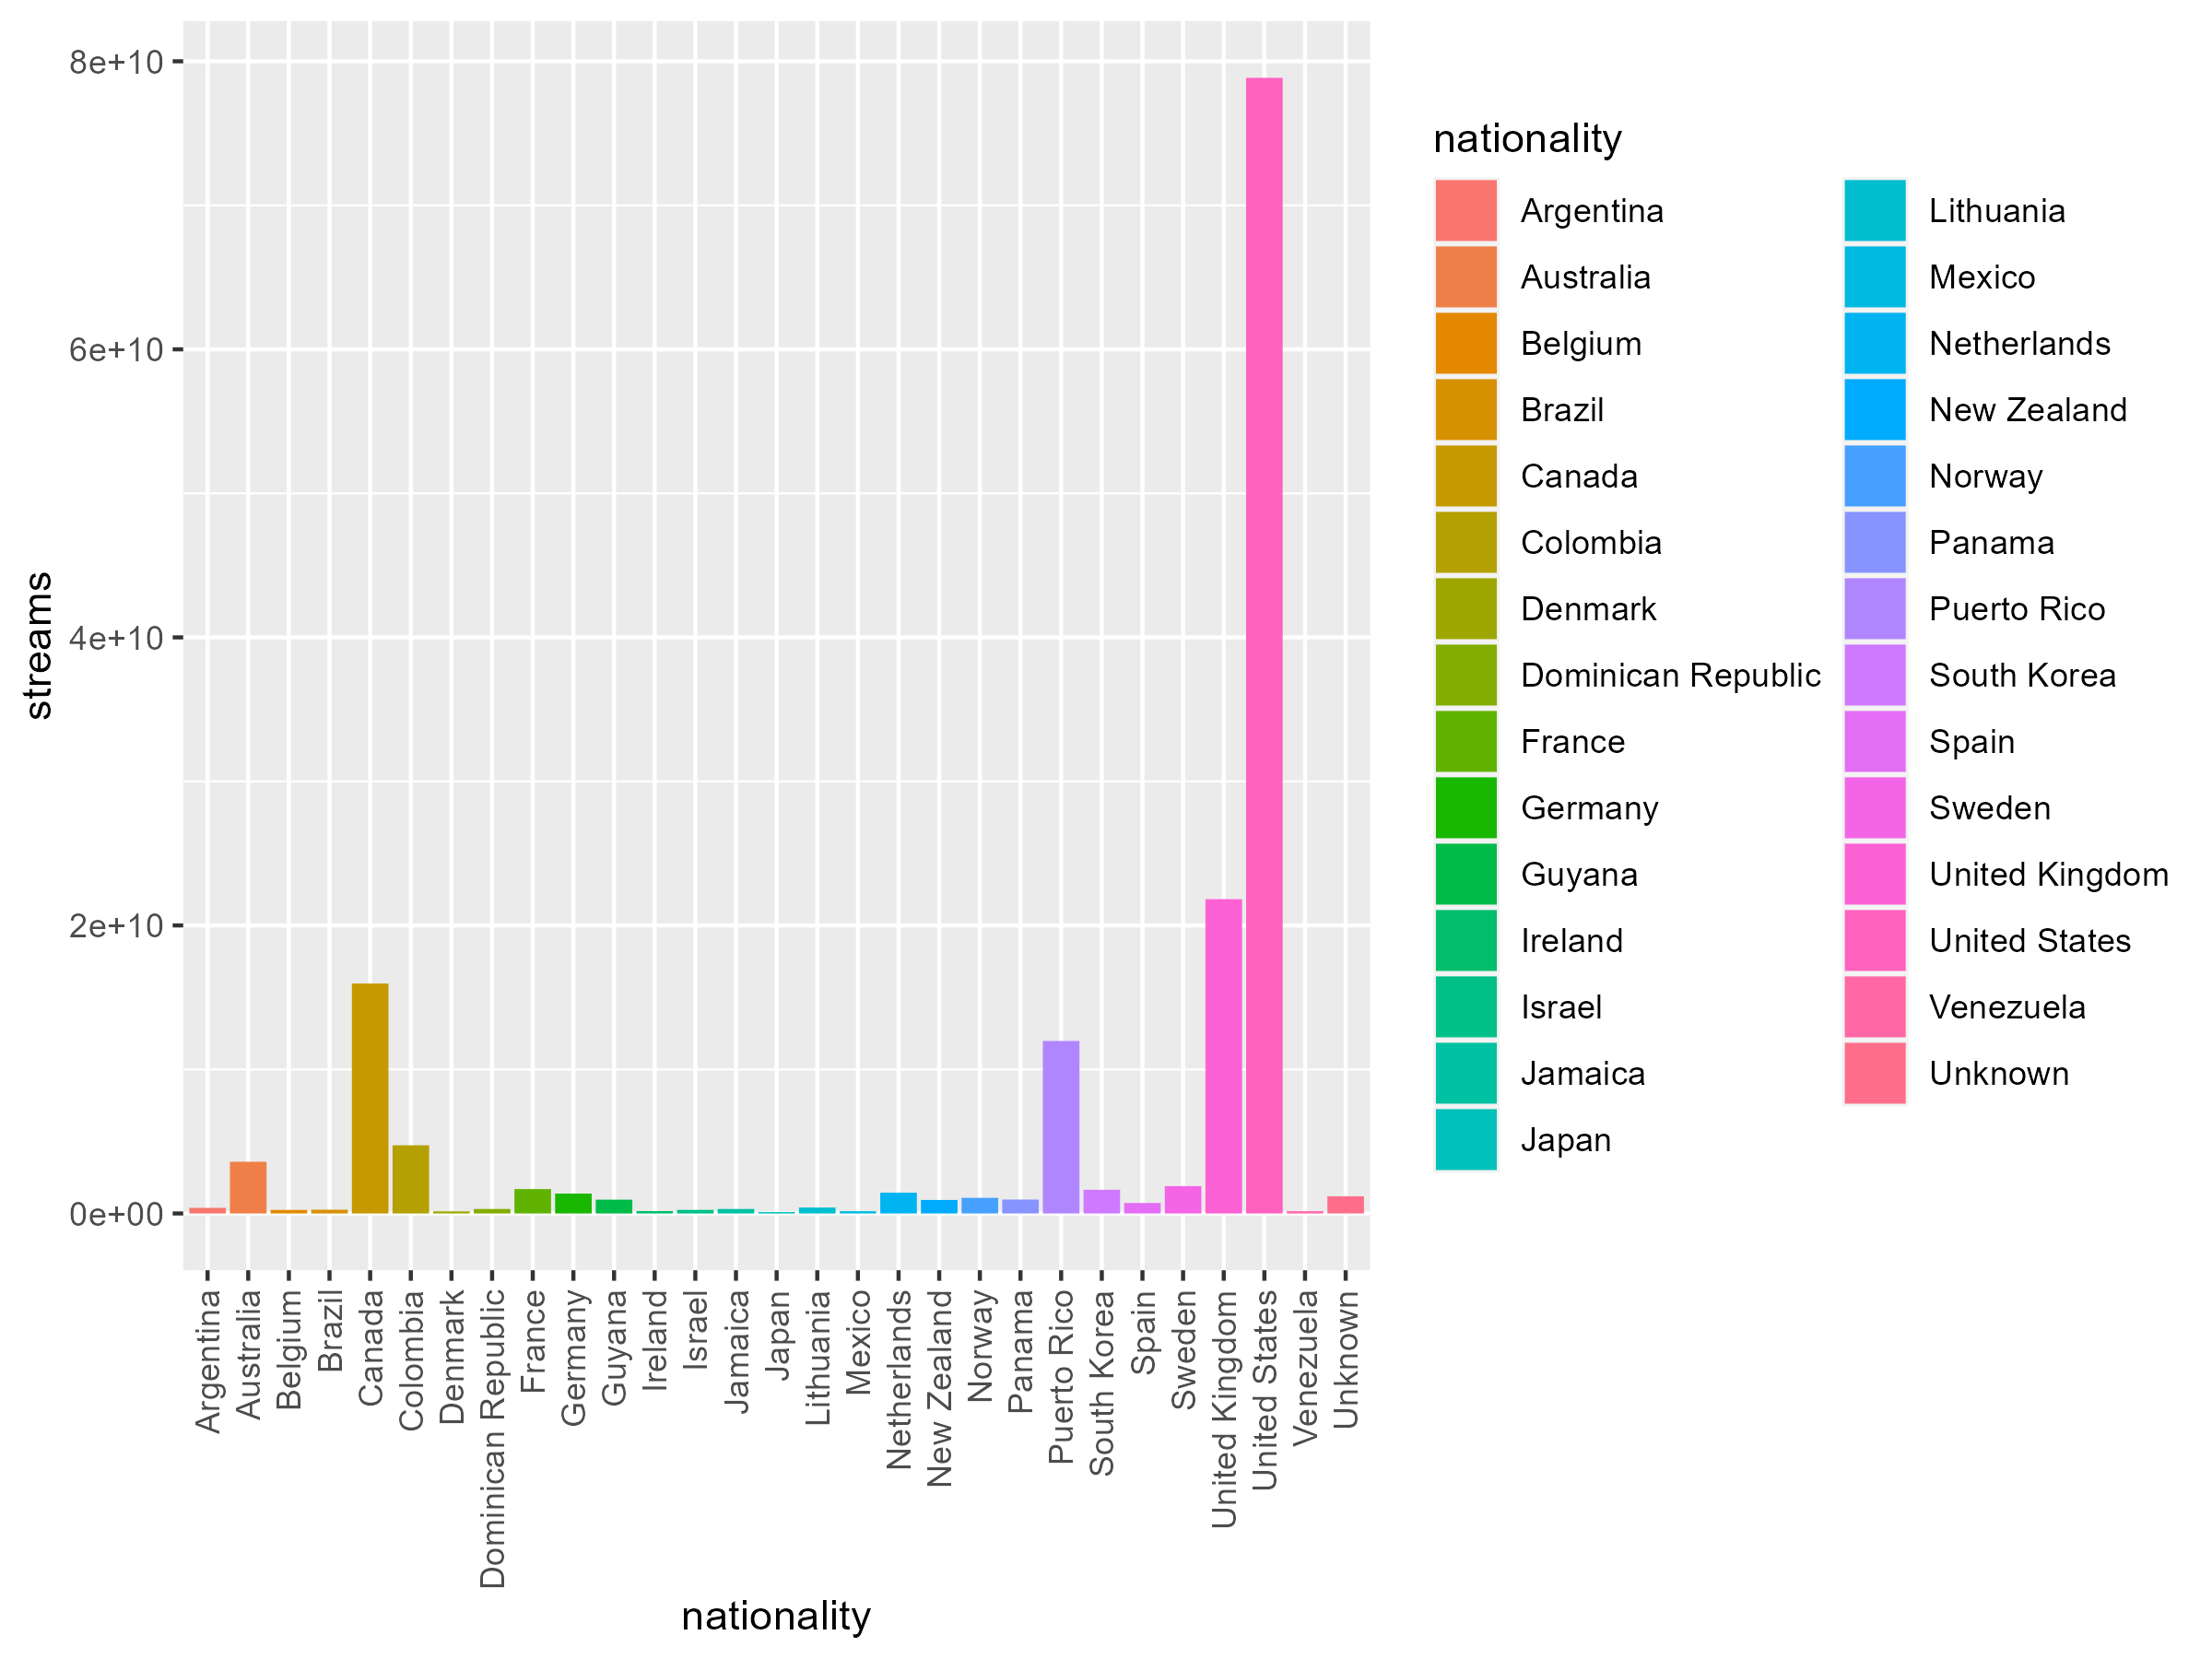
\includegraphics[width=0.95\linewidth]{Images/3_Preprocessing/nationalitystreams.png}
        \caption{Bar plot de \textit{nationality} amb \textit{streams}}
        \label{fig:BivariateP_nationstreams}
    \end{minipage}%
    \begin{minipage}{.4\textwidth}
        \centering
        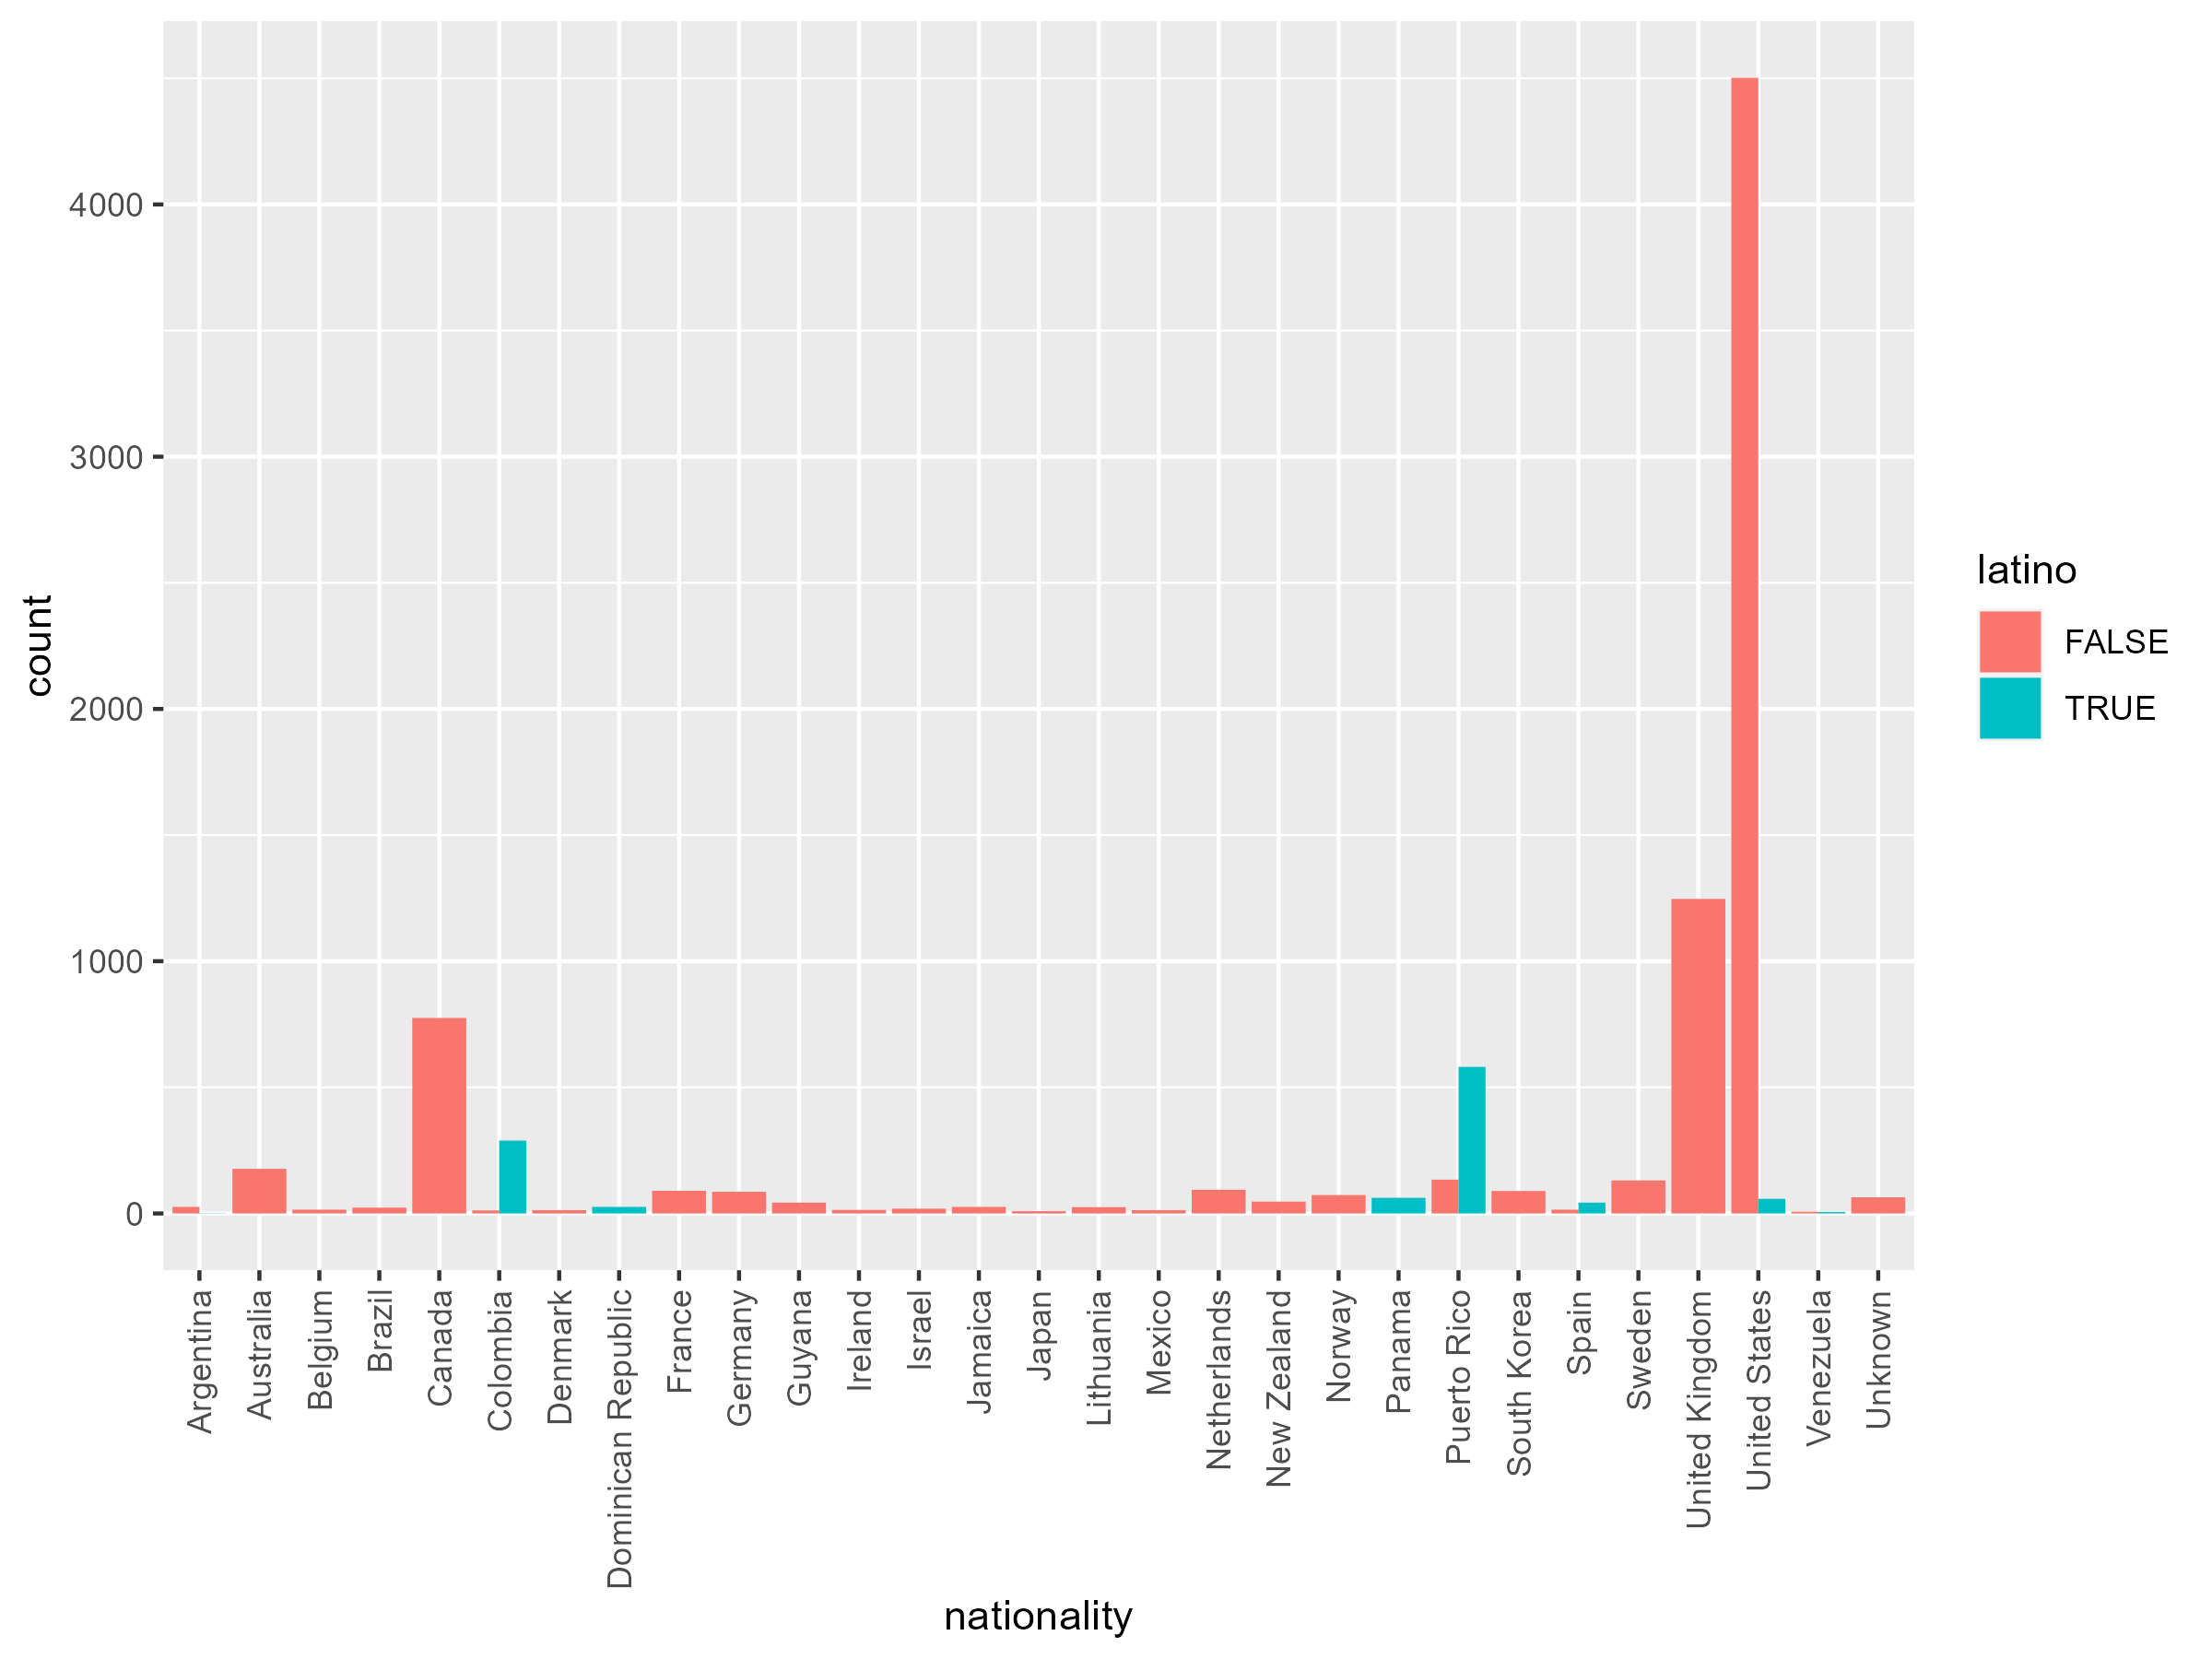
\includegraphics[width=0.95\linewidth]{Images/3_Preprocessing/nationalitylatino.png}
        \caption{Bar plot de \textit{nationality} amb \textit{latino}}
        \label{fig:BivariateP_nationlati}
    \end{minipage}%
\end{figure}

\subsection{Ampliació de la base de dades mitjançants APIs}

Com ja s'ha mencionat anteriorment, la nostra base de dades originària de \textbf{Kaggle} incloïa diverses variables sobre cançons com ara la seva llargada, timbre, duració, etc. Després d'un primer preprocessament on es van eliminar totes les aparicions de les cançons si l'artista no era el principal, ens vam centrar més en els artistes, ja que l'anàlisi resultava més interessant i prometedor. La falta d'informació detallada sobre els artistes ens va portar a utilitzar diferents APIs per a enriquir el nostre conjunt de dades.

\subsubsection{Selecció d'APIs}

Per a millorar la qualitat i riquesa de les dades, es va decidir incorporar informació addicional sobre els artistes, com ara la seva ubicació \textbf{(País / Ciutat)}, gènere \textbf{(Masculí / Femení / No binari)} i si l'artista és un \textbf{individu} o un \textbf{grup}. A més, també es va incorporar la lletra de les cançons per tal de poder realitzar un \textit{text analysis} més endavant.. Això es va aconseguir mitjançant l'ús de diverses APIs públiques:
\begin{itemize}
    \item \textbf{MusicBrainz API}: Per obtenir detalls específics dels artistes, incloent si són solistes o grups, i el gènere del grup basat en els seus membres.
    \item \textbf{CountriesNow API}: Per verificar si una ciutat determinada es troba dins d'un país específic, evitant així inconsistències en la ubicació.
    \item \textbf{RestCountries API}: Per obtenir la capital d'un país quan la ciutat de l'artista no està disponible o no es pot verificar correctament.
    \item \textbf{Genius API}: Per obtenir els lyrics de les cançons. S'ha usat amb la llibreria de \textit{Python} \textit{lyricsgenius} .
\end{itemize}

\subsubsection{Gestió d'errors i tècniques de millora}

Per a assegurar la fiabilitat i precisió de les dades recopilades, es van implementar diverses estratègies:
\begin{itemize}
    \item Esperar un temps prudencial entre trucades a la API per evitar sobrecàrregues i possibles bloquejos.
    \item Realitzar múltiples intents per cada trucada a l'API, gestionant els errors temporals de manera eficient.
    \item Substituir els valors no disponibles (\textit{NA}) per les capitals dels països corresponents quan la informació de la ciutat de l'artista no es trobava o era incorrecta.
    \item Verificació manual per a casos on les dades automàticament recollides no eren coherents, com ara ciutats que no pertanyien al país indicat o països erròniament identificats com a ciutats.
\end{itemize}

Malgrat l'aplicació d'aquestes mesures, alguns errors en la localització d'artistes van requerir correccions manuals, especialment en casos on les ciutats no concordaven amb els països o quan la informació retornada per les APIs era incorrecta a causa de la confusió amb altres artistes de nom similar. Aquestes situacions van ser poc freqüents però destacables, ja que reflecteixen les limitacions inherents a l'ús de dades automàticament recollides i la importància de la revisió humana en la curació de conjunts de dades.

\subsubsection{Resultats}

Després de l'execució de l'script i la implementació de les tècniques esmentades, es va obtenir un conjunt de dades considerablement millorat, amb informació més completa i precisa sobre els artistes i amb les lletres de les cançons. Aquest enriquiment de les dades obre noves possibilitats per a l'anàlisi, permetent estudis més detallats i específics sobre la música i els seus creadors en la plataforma Spotify.


